\documentclass[11pt]{article}
% Build: cd paper && latexmk -pdf paper.tex   (tables and numbers: python3 make_tables.py)
\usepackage[T1]{fontenc}
\usepackage{lmodern}
\usepackage[margin=1in]{geometry}
\usepackage{microtype}
\usepackage{amsmath}
\usepackage{booktabs}
\usepackage{threeparttable}
\usepackage{caption}
\usepackage{setspace}
\usepackage{pgfplots}
\pgfplotsset{compat=1.18}
\usetikzlibrary{patterns}
\usepackage[authoryear,round]{natbib}
\usepackage[hidelinks]{hyperref}
\usepackage{xurl}
\usepackage{fvextra}
\usepackage{float}
\usepackage{placeins}

\captionsetup{font=small,labelfont=bf,skip=4pt}
\setstretch{1.08}
\setlength{\parskip}{0.35em}
\newcommand{\tabnote}[1]{\par\vspace{3pt}\begin{minipage}{\linewidth}\footnotesize\setstretch{1.0}#1\end{minipage}}

% generated by paper/make_tables.py - do not edit
% generated by paper/make_tables.py - every number quoted in the text
\makeatletter
\newcommand{\R}[1]{\@ifundefined{R@#1}{\textbf{??#1??}\PackageWarning{numbers}{undefined key #1}}{\@nameuse{R@#1}}}
\@namedef{R@all.fable.MPS.t}{3.02}
\@namedef{R@all.fable.d10.t}{1.44}
\@namedef{R@all.fable.d2.t}{1.41}
\@namedef{R@all.fable.t10.t}{2.52}
\@namedef{R@all.fable.t2.t}{2.69}
\@namedef{R@all.gemini.MPS.t}{1.36}
\@namedef{R@all.gemini.d10.t}{$-$0.97}
\@namedef{R@all.gemini.d2.t}{$-$0.95}
\@namedef{R@all.gemini.t10.t}{0.23}
\@namedef{R@all.gemini.t2.t}{0.50}
\@namedef{R@allctrl.fable.MPS.t}{2.27}
\@namedef{R@allctrl.fable.t10.t}{2.26}
\@namedef{R@allctrl.fable.t2.t}{2.21}
\@namedef{R@allctrl.gemini.MPS.t}{$-$0.45}
\@namedef{R@alpha.fable.chg}{0.921}
\@namedef{R@alpha.fable.drop}{2\%}
\@namedef{R@alpha.fable.hold}{0.928}
\@namedef{R@alpha.fable.raw}{0.953}
\@namedef{R@alpha.fable.resid}{0.930}
\@namedef{R@alpha.fablefull.chg}{0.896}
\@namedef{R@alpha.fablefull.drop}{2\%}
\@namedef{R@alpha.fablefull.hold}{0.950}
\@namedef{R@alpha.fablefull.raw}{0.972}
\@namedef{R@alpha.fablefull.resid}{0.957}
\@namedef{R@alpha.gem.chg}{0.698}
\@namedef{R@alpha.gem.drop}{29\%}
\@namedef{R@alpha.gem.hold}{0.524}
\@namedef{R@alpha.gem.raw}{0.791}
\@namedef{R@alpha.gem.resid}{0.564}
\@namedef{R@alpha.gem04.chg}{0.697}
\@namedef{R@alpha.gem04.drop}{7\%}
\@namedef{R@alpha.gem04.hold}{0.885}
\@namedef{R@alpha.gem04.raw}{0.891}
\@namedef{R@alpha.gem04.resid}{0.831}
\@namedef{R@alpha.gemfull.chg}{0.729}
\@namedef{R@alpha.gemfull.drop}{6\%}
\@namedef{R@alpha.gemfull.hold}{0.881}
\@namedef{R@alpha.gemfull.raw}{0.933}
\@namedef{R@alpha.gemfull.resid}{0.874}
\@namedef{R@alpha.haiku.chg}{0.422}
\@namedef{R@alpha.haiku.drop}{16\%}
\@namedef{R@alpha.haiku.hold}{0.084}
\@namedef{R@alpha.haiku.raw}{0.398}
\@namedef{R@alpha.haiku.resid}{0.336}
\@namedef{R@alpha.mini.chg}{0.579}
\@namedef{R@alpha.mini.drop}{18\%}
\@namedef{R@alpha.mini.hold}{0.355}
\@namedef{R@alpha.mini.raw}{0.634}
\@namedef{R@alpha.mini.resid}{0.519}
\@namedef{R@base.adj}{181}
\@namedef{R@base.br}{89}
\@namedef{R@base.brpct}{43\%}
\@namedef{R@base.n}{206}
\@namedef{R@base.w1}{106}
\@namedef{R@base.w1pct}{51\%}
\@namedef{R@base.w3}{190}
\@namedef{R@base.w3pct}{92\%}
\@namedef{R@base.zlb.br}{28}
\@namedef{R@base.zlb.w3}{54}
\@namedef{R@bench.after}{1.15}
\@namedef{R@bench.full}{2.75}
\@namedef{R@bench.share}{0.49}
\@namedef{R@bench.sharepct}{49\%}
\@namedef{R@beyond.fable.gainmax}{0.64}
\@namedef{R@beyond.fable.gainmin}{0.04}
\@namedef{R@beyond.fable.tmax}{1.06}
\@namedef{R@beyond.gainmax}{1.05}
\@namedef{R@block.cuts}{3}
\@namedef{R@block.hikes}{9}
\@namedef{R@corpus.files}{228}
\@namedef{R@corpus.first}{2000-02-02}
\@namedef{R@corpus.last}{2026-07-29}
\@namedef{R@corpus.multimonth}{7}
\@namedef{R@corpus.notice}{7}
\@namedef{R@corpus.policy}{221}
\@namedef{R@corpus.policy.check}{221}
\@namedef{R@corpus.prenotices}{6}
\@namedef{R@corpus.scheduled}{212}
\@namedef{R@corpus.unscheduledpolicy}{2}
\@namedef{R@corpus.unscheduledrate}{7}
\@namedef{R@corpus.zlbnotices}{1}
\@namedef{R@corr.clean.blind}{0.913}
\@namedef{R@corr.clean.para}{0.796}
\@namedef{R@corr.fable.blind}{0.916}
\@namedef{R@corr.fable.clean}{0.942}
\@namedef{R@corr.fable.dict}{0.424}
\@namedef{R@corr.fable.gemini}{0.739}
\@namedef{R@corr.fable.gpt4}{0.568}
\@namedef{R@corr.fable.para}{0.824}
\@namedef{R@corr.gemini.gpt4}{0.691}
\@namedef{R@cover.fable.fewer}{47}
\@namedef{R@cover.fable.fewfirst}{2020}
\@namedef{R@cover.fable.five}{174}
\@namedef{R@cover.fable.none}{0}
\@namedef{R@cover.fable.prefewer}{33}
\@namedef{R@cover.fable.prefive}{167}
\@namedef{R@cover.gemini.fewer}{0}
\@namedef{R@cover.gemini.five}{221}
\@namedef{R@cover.gemini.none}{0}
\@namedef{R@cover.gemini.prefewer}{0}
\@namedef{R@cover.gemini.prefive}{200}
\@namedef{R@desc.corr.MPS.t10}{0.70}
\@namedef{R@desc.corr.MPS.t2}{0.94}
\@namedef{R@desc.corr.t10.d10}{0.67}
\@namedef{R@desc.corr.t2.d2}{0.64}
\@namedef{R@desc.hold}{132}
\@namedef{R@desc.moves}{68}
\@namedef{R@desc.n.MPS}{132}
\@namedef{R@desc.n.MPS_ORTH}{125}
\@namedef{R@desc.n.d10}{120}
\@namedef{R@desc.n.d2}{120}
\@namedef{R@desc.n.t10}{132}
\@namedef{R@desc.n.t2}{132}
\@namedef{R@desc.post}{21}
\@namedef{R@desc.pre}{200}
\@namedef{R@desc.prepairs}{199}
\@namedef{R@desc.sd.MPS}{0.039}
\@namedef{R@desc.sd.MPS_ORTH}{0.041}
\@namedef{R@desc.sd.d10}{8.0}
\@namedef{R@desc.sd.d2}{6.1}
\@namedef{R@desc.sd.t10}{4.4}
\@namedef{R@desc.sd.t2}{4.4}
\@namedef{R@dummy.cheap.max}{39\%}
\@namedef{R@dummy.cheap.min}{26\%}
\@namedef{R@dummy.fable.drop}{3\%}
\@namedef{R@dummy.fable.resid}{0.930}
\@namedef{R@dummy.gem.drop}{31\%}
\@namedef{R@dummy.gem.resid}{0.557}
\@namedef{R@dummy.haiku.drop}{39\%}
\@namedef{R@dummy.haiku.resid}{0.371}
\@namedef{R@dummy.mini.drop}{26\%}
\@namedef{R@dummy.mini.resid}{0.541}
\@namedef{R@extra.decblind.n}{132}
\@namedef{R@extra.decblind.p}{0.070}
\@namedef{R@extra.decblind.t}{1.83}
\@namedef{R@extra.decblindres.n}{132}
\@namedef{R@extra.decblindres.p}{0.026}
\@namedef{R@extra.decblindres.t}{2.25}
\@namedef{R@extra.decpara.n}{132}
\@namedef{R@extra.decpara.p}{0.331}
\@namedef{R@extra.decpara.t}{0.98}
\@namedef{R@extra.decparares.n}{132}
\@namedef{R@extra.decparares.p}{$<$0.001}
\@namedef{R@extra.decparares.t}{3.59}
\@namedef{R@extra.lagds.n}{132}
\@namedef{R@extra.lagds.p}{0.024}
\@namedef{R@extra.lagds.t}{2.29}
\@namedef{R@extra.lagmps.n}{132}
\@namedef{R@extra.lagmps.p}{0.019}
\@namedef{R@extra.lagmps.t}{2.39}
\@namedef{R@extra.level.n}{132}
\@namedef{R@extra.level.p}{0.170}
\@namedef{R@extra.level.t}{1.38}
\@namedef{R@extra.predpart.n}{125}
\@namedef{R@extra.predpart.p}{$<$0.001}
\@namedef{R@extra.predpart.t}{4.99}
\@namedef{R@extra.predsame.n}{125}
\@namedef{R@extra.predsame.p}{0.018}
\@namedef{R@extra.predsame.t}{2.39}
\@namedef{R@extra.sub0007.n}{32}
\@namedef{R@extra.sub0007.p}{0.196}
\@namedef{R@extra.sub0007.t}{1.32}
\@namedef{R@extra.sub0815.n}{58}
\@namedef{R@extra.sub0815.p}{0.673}
\@namedef{R@extra.sub0815.t}{0.42}
\@namedef{R@extra.sub1623.n}{42}
\@namedef{R@extra.sub1623.p}{0.002}
\@namedef{R@extra.sub1623.t}{3.40}
\@namedef{R@extra.winsor.n}{132}
\@namedef{R@extra.winsor.p}{0.012}
\@namedef{R@extra.winsor.t}{2.54}
\@namedef{R@fable.sd}{0.243}
\@namedef{R@fable.zero}{5}
\@namedef{R@fable.zeron}{132}
\@namedef{R@fam.MPS.all.ctrl.beta}{0.036}
\@namedef{R@fam.MPS.all.ctrl.bonf}{0.294}
\@namedef{R@fam.MPS.all.ctrl.holm}{0.245}
\@namedef{R@fam.MPS.all.ctrl.n}{198}
\@namedef{R@fam.MPS.all.ctrl.p}{0.025}
\@namedef{R@fam.MPS.all.ctrl.t}{2.27}
\@namedef{R@fam.MPS.all.none.beta}{0.049}
\@namedef{R@fam.MPS.all.none.bonf}{0.034}
\@namedef{R@fam.MPS.all.none.holm}{0.034}
\@namedef{R@fam.MPS.all.none.n}{198}
\@namedef{R@fam.MPS.all.none.p}{0.003}
\@namedef{R@fam.MPS.all.none.t}{3.02}
\@namedef{R@fam.MPS.hold.none.beta}{0.033}
\@namedef{R@fam.MPS.hold.none.bonf}{0.217}
\@namedef{R@fam.MPS.hold.none.holm}{0.199}
\@namedef{R@fam.MPS.hold.none.n}{132}
\@namedef{R@fam.MPS.hold.none.p}{0.018}
\@namedef{R@fam.MPS.hold.none.t}{2.39}
\@namedef{R@fam.MPS_ORTH.all.ctrl.beta}{0.010}
\@namedef{R@fam.MPS_ORTH.all.ctrl.bonf}{1.000}
\@namedef{R@fam.MPS_ORTH.all.ctrl.holm}{1.000}
\@namedef{R@fam.MPS_ORTH.all.ctrl.n}{189}
\@namedef{R@fam.MPS_ORTH.all.ctrl.p}{0.578}
\@namedef{R@fam.MPS_ORTH.all.ctrl.t}{0.56}
\@namedef{R@fam.MPS_ORTH.all.none.beta}{0.014}
\@namedef{R@fam.MPS_ORTH.all.none.bonf}{1.000}
\@namedef{R@fam.MPS_ORTH.all.none.holm}{1.000}
\@namedef{R@fam.MPS_ORTH.all.none.n}{189}
\@namedef{R@fam.MPS_ORTH.all.none.p}{0.431}
\@namedef{R@fam.MPS_ORTH.all.none.t}{0.79}
\@namedef{R@fam.MPS_ORTH.hold.none.beta}{0.011}
\@namedef{R@fam.MPS_ORTH.hold.none.bonf}{1.000}
\@namedef{R@fam.MPS_ORTH.hold.none.holm}{1.000}
\@namedef{R@fam.MPS_ORTH.hold.none.n}{125}
\@namedef{R@fam.MPS_ORTH.hold.none.p}{0.490}
\@namedef{R@fam.MPS_ORTH.hold.none.t}{0.69}
\@namedef{R@fam.d10.all.ctrl.beta}{4.39}
\@namedef{R@fam.d10.all.ctrl.bonf}{1.000}
\@namedef{R@fam.d10.all.ctrl.holm}{1.000}
\@namedef{R@fam.d10.all.ctrl.n}{173}
\@namedef{R@fam.d10.all.ctrl.p}{0.130}
\@namedef{R@fam.d10.all.ctrl.t}{1.52}
\@namedef{R@fam.d10.all.none.beta}{4.27}
\@namedef{R@fam.d10.all.none.bonf}{1.000}
\@namedef{R@fam.d10.all.none.holm}{1.000}
\@namedef{R@fam.d10.all.none.n}{173}
\@namedef{R@fam.d10.all.none.p}{0.151}
\@namedef{R@fam.d10.all.none.t}{1.44}
\@namedef{R@fam.d10.hold.none.beta}{5.20}
\@namedef{R@fam.d10.hold.none.bonf}{1.000}
\@namedef{R@fam.d10.hold.none.holm}{0.756}
\@namedef{R@fam.d10.hold.none.n}{120}
\@namedef{R@fam.d10.hold.none.p}{0.084}
\@namedef{R@fam.d10.hold.none.t}{1.74}
\@namedef{R@fam.d2.all.ctrl.beta}{4.93}
\@namedef{R@fam.d2.all.ctrl.bonf}{1.000}
\@namedef{R@fam.d2.all.ctrl.holm}{1.000}
\@namedef{R@fam.d2.all.ctrl.n}{173}
\@namedef{R@fam.d2.all.ctrl.p}{0.160}
\@namedef{R@fam.d2.all.ctrl.t}{1.41}
\@namedef{R@fam.d2.all.none.beta}{5.02}
\@namedef{R@fam.d2.all.none.bonf}{1.000}
\@namedef{R@fam.d2.all.none.holm}{1.000}
\@namedef{R@fam.d2.all.none.n}{173}
\@namedef{R@fam.d2.all.none.p}{0.162}
\@namedef{R@fam.d2.all.none.t}{1.41}
\@namedef{R@fam.d2.hold.none.beta}{3.77}
\@namedef{R@fam.d2.hold.none.bonf}{1.000}
\@namedef{R@fam.d2.hold.none.holm}{1.000}
\@namedef{R@fam.d2.hold.none.n}{120}
\@namedef{R@fam.d2.hold.none.p}{0.306}
\@namedef{R@fam.d2.hold.none.t}{1.03}
\@namedef{R@fred.days}{1229}
\@namedef{R@fred.first}{2021-10-06}
\@namedef{R@fred.last}{2026-09-08}
\@namedef{R@g.MPS.blind.z}{1.45}
\@namedef{R@g.MPS.para.z}{1.26}
\@namedef{R@g.d10.blind.z}{1.54}
\@namedef{R@g.d10.para.z}{0.97}
\@namedef{R@g.d2.blind.z}{2.15}
\@namedef{R@g.d2.para.z}{1.70}
\@namedef{R@g.n}{6}
\@namedef{R@g.over196}{1}
\@namedef{R@g.zmax}{2.15}
\@namedef{R@g.zmin}{0.97}
\@namedef{R@gemini.sd}{0.301}
\@namedef{R@gpt4.atminus1}{98}
\@namedef{R@gpt4.atminus1pct}{44\%}
\@namedef{R@gpt4.distinct}{10}
\@namedef{R@gpt4.nscores}{225}
\@namedef{R@gpt4.sd}{0.388}
\@namedef{R@gpt4.zero}{86}
\@namedef{R@gpt4.zeron}{129}
\@namedef{R@gpt4.zeropct}{67\%}
\@namedef{R@gpt4.zlbfloor}{40}
\@namedef{R@gpt4.zlbn}{56}
\@namedef{R@h.fable.MPS.all-post.n}{18}
\@namedef{R@h.fable.MPS.all-post.t}{2.16}
\@namedef{R@h.fable.d10.all-post.n}{39}
\@namedef{R@h.fable.d10.all-post.t}{1.77}
\@namedef{R@h.fable.d10.hold-post.n}{22}
\@namedef{R@h.fable.d10.hold-post.t}{2.37}
\@namedef{R@h.fable.d2.all-post.n}{39}
\@namedef{R@h.fable.d2.all-post.t}{1.90}
\@namedef{R@h.fable.d2.hold-post.n}{22}
\@namedef{R@h.fable.d2.hold-post.t}{1.90}
\@namedef{R@h.gpt4.MPS.all-post.n}{18}
\@namedef{R@h.gpt4.MPS.all-post.t}{$-$0.31}
\@namedef{R@h.gpt4.MPS.all-pre.n}{175}
\@namedef{R@h.gpt4.MPS.all-pre.t}{0.57}
\@namedef{R@h.gpt4.MPS.hold-pre.n}{122}
\@namedef{R@h.gpt4.MPS.hold-pre.t}{$-$0.24}
\@namedef{R@h.gpt4.d10.all-post.n}{39}
\@namedef{R@h.gpt4.d10.all-post.t}{$-$0.18}
\@namedef{R@h.gpt4.d10.all-pre.n}{150}
\@namedef{R@h.gpt4.d10.all-pre.t}{$-$1.12}
\@namedef{R@h.gpt4.d10.hold-post.n}{22}
\@namedef{R@h.gpt4.d10.hold-post.t}{1.33}
\@namedef{R@h.gpt4.d10.hold-pre.n}{110}
\@namedef{R@h.gpt4.d10.hold-pre.t}{$-$0.95}
\@namedef{R@h.gpt4.d2.all-post.n}{39}
\@namedef{R@h.gpt4.d2.all-post.t}{$-$0.09}
\@namedef{R@h.gpt4.d2.all-pre.n}{150}
\@namedef{R@h.gpt4.d2.all-pre.t}{$-$1.79}
\@namedef{R@h.gpt4.d2.hold-post.n}{22}
\@namedef{R@h.gpt4.d2.hold-post.t}{0.56}
\@namedef{R@h.gpt4.d2.hold-pre.n}{110}
\@namedef{R@h.gpt4.d2.hold-pre.t}{$-$3.33}
\@namedef{R@hold.blind.MPS.beta}{0.017}
\@namedef{R@hold.blind.MPS.n}{132}
\@namedef{R@hold.blind.MPS.p}{0.156}
\@namedef{R@hold.blind.MPS.t}{1.43}
\@namedef{R@hold.blind.MPS_ORTH.beta}{$-$0.001}
\@namedef{R@hold.blind.MPS_ORTH.n}{125}
\@namedef{R@hold.blind.MPS_ORTH.p}{0.956}
\@namedef{R@hold.blind.MPS_ORTH.t}{$-$0.06}
\@namedef{R@hold.blind.d10.beta}{1.44}
\@namedef{R@hold.blind.d10.n}{120}
\@namedef{R@hold.blind.d10.p}{0.546}
\@namedef{R@hold.blind.d10.t}{0.61}
\@namedef{R@hold.blind.d2.beta}{0.06}
\@namedef{R@hold.blind.d2.n}{120}
\@namedef{R@hold.blind.d2.p}{0.984}
\@namedef{R@hold.blind.d2.t}{0.02}
\@namedef{R@hold.blind.t10.beta}{1.45}
\@namedef{R@hold.blind.t10.n}{132}
\@namedef{R@hold.blind.t10.p}{0.170}
\@namedef{R@hold.blind.t10.t}{1.38}
\@namedef{R@hold.blind.t2.beta}{1.72}
\@namedef{R@hold.blind.t2.n}{132}
\@namedef{R@hold.blind.t2.p}{0.265}
\@namedef{R@hold.blind.t2.t}{1.12}
\@namedef{R@hold.clean.MPS.beta}{0.026}
\@namedef{R@hold.clean.MPS.n}{132}
\@namedef{R@hold.clean.MPS.p}{0.030}
\@namedef{R@hold.clean.MPS.t}{2.20}
\@namedef{R@hold.clean.MPS_ORTH.beta}{0.008}
\@namedef{R@hold.clean.MPS_ORTH.n}{125}
\@namedef{R@hold.clean.MPS_ORTH.p}{0.582}
\@namedef{R@hold.clean.MPS_ORTH.t}{0.55}
\@namedef{R@hold.clean.d10.beta}{3.18}
\@namedef{R@hold.clean.d10.n}{120}
\@namedef{R@hold.clean.d10.p}{0.165}
\@namedef{R@hold.clean.d10.t}{1.40}
\@namedef{R@hold.clean.d2.beta}{2.21}
\@namedef{R@hold.clean.d2.n}{120}
\@namedef{R@hold.clean.d2.p}{0.462}
\@namedef{R@hold.clean.d2.t}{0.74}
\@namedef{R@hold.clean.t10.beta}{1.85}
\@namedef{R@hold.clean.t10.n}{132}
\@namedef{R@hold.clean.t10.p}{0.082}
\@namedef{R@hold.clean.t10.t}{1.75}
\@namedef{R@hold.clean.t2.beta}{2.66}
\@namedef{R@hold.clean.t2.n}{132}
\@namedef{R@hold.clean.t2.p}{0.084}
\@namedef{R@hold.clean.t2.t}{1.74}
\@namedef{R@hold.dict.MPS.beta}{$-$0.010}
\@namedef{R@hold.dict.MPS.n}{132}
\@namedef{R@hold.dict.MPS.p}{0.323}
\@namedef{R@hold.dict.MPS.t}{$-$0.99}
\@namedef{R@hold.dict.MPS_ORTH.beta}{$-$0.021}
\@namedef{R@hold.dict.MPS_ORTH.n}{125}
\@namedef{R@hold.dict.MPS_ORTH.p}{0.083}
\@namedef{R@hold.dict.MPS_ORTH.t}{$-$1.75}
\@namedef{R@hold.dict.d10.beta}{1.70}
\@namedef{R@hold.dict.d10.n}{120}
\@namedef{R@hold.dict.d10.p}{0.388}
\@namedef{R@hold.dict.d10.t}{0.87}
\@namedef{R@hold.dict.d2.beta}{$-$0.36}
\@namedef{R@hold.dict.d2.n}{120}
\@namedef{R@hold.dict.d2.p}{0.866}
\@namedef{R@hold.dict.d2.t}{$-$0.17}
\@namedef{R@hold.dict.t10.beta}{$-$0.54}
\@namedef{R@hold.dict.t10.n}{132}
\@namedef{R@hold.dict.t10.p}{0.510}
\@namedef{R@hold.dict.t10.t}{$-$0.66}
\@namedef{R@hold.dict.t2.beta}{$-$1.52}
\@namedef{R@hold.dict.t2.n}{132}
\@namedef{R@hold.dict.t2.p}{0.167}
\@namedef{R@hold.dict.t2.t}{$-$1.39}
\@namedef{R@hold.fable.MPS.beta}{0.033}
\@namedef{R@hold.fable.MPS.n}{132}
\@namedef{R@hold.fable.MPS.p}{0.018}
\@namedef{R@hold.fable.MPS.t}{2.39}
\@namedef{R@hold.fable.MPS_ORTH.beta}{0.011}
\@namedef{R@hold.fable.MPS_ORTH.n}{125}
\@namedef{R@hold.fable.MPS_ORTH.p}{0.490}
\@namedef{R@hold.fable.MPS_ORTH.t}{0.69}
\@namedef{R@hold.fable.d10.beta}{5.20}
\@namedef{R@hold.fable.d10.n}{120}
\@namedef{R@hold.fable.d10.p}{0.084}
\@namedef{R@hold.fable.d10.t}{1.74}
\@namedef{R@hold.fable.d2.beta}{3.77}
\@namedef{R@hold.fable.d2.n}{120}
\@namedef{R@hold.fable.d2.p}{0.306}
\@namedef{R@hold.fable.d2.t}{1.03}
\@namedef{R@hold.fable.t10.beta}{2.98}
\@namedef{R@hold.fable.t10.n}{132}
\@namedef{R@hold.fable.t10.p}{0.037}
\@namedef{R@hold.fable.t10.t}{2.10}
\@namedef{R@hold.fable.t2.beta}{3.76}
\@namedef{R@hold.fable.t2.n}{132}
\@namedef{R@hold.fable.t2.p}{0.042}
\@namedef{R@hold.fable.t2.t}{2.05}
\@namedef{R@hold.gemini.MPS.beta}{0.003}
\@namedef{R@hold.gemini.MPS.n}{132}
\@namedef{R@hold.gemini.MPS.p}{0.786}
\@namedef{R@hold.gemini.MPS.t}{0.27}
\@namedef{R@hold.gemini.MPS_ORTH.beta}{$-$0.009}
\@namedef{R@hold.gemini.MPS_ORTH.n}{125}
\@namedef{R@hold.gemini.MPS_ORTH.p}{0.367}
\@namedef{R@hold.gemini.MPS_ORTH.t}{$-$0.91}
\@namedef{R@hold.gemini.d10.beta}{$-$0.15}
\@namedef{R@hold.gemini.d10.n}{120}
\@namedef{R@hold.gemini.d10.p}{0.913}
\@namedef{R@hold.gemini.d10.t}{$-$0.11}
\@namedef{R@hold.gemini.d2.beta}{$-$2.26}
\@namedef{R@hold.gemini.d2.n}{120}
\@namedef{R@hold.gemini.d2.p}{0.200}
\@namedef{R@hold.gemini.d2.t}{$-$1.29}
\@namedef{R@hold.gemini.t10.beta}{0.06}
\@namedef{R@hold.gemini.t10.n}{132}
\@namedef{R@hold.gemini.t10.p}{0.924}
\@namedef{R@hold.gemini.t10.t}{0.10}
\@namedef{R@hold.gemini.t2.beta}{0.03}
\@namedef{R@hold.gemini.t2.n}{132}
\@namedef{R@hold.gemini.t2.p}{0.977}
\@namedef{R@hold.gemini.t2.t}{0.03}
\@namedef{R@hold.gpt4.MPS.beta}{$-$0.006}
\@namedef{R@hold.gpt4.MPS.n}{129}
\@namedef{R@hold.gpt4.MPS.p}{0.527}
\@namedef{R@hold.gpt4.MPS.t}{$-$0.63}
\@namedef{R@hold.gpt4.MPS_ORTH.beta}{$-$0.016}
\@namedef{R@hold.gpt4.MPS_ORTH.n}{122}
\@namedef{R@hold.gpt4.MPS_ORTH.p}{0.058}
\@namedef{R@hold.gpt4.MPS_ORTH.t}{$-$1.92}
\@namedef{R@hold.gpt4.d10.beta}{$-$0.05}
\@namedef{R@hold.gpt4.d10.n}{117}
\@namedef{R@hold.gpt4.d10.p}{0.969}
\@namedef{R@hold.gpt4.d10.t}{$-$0.04}
\@namedef{R@hold.gpt4.d2.beta}{$-$2.55}
\@namedef{R@hold.gpt4.d2.n}{117}
\@namedef{R@hold.gpt4.d2.p}{0.062}
\@namedef{R@hold.gpt4.d2.t}{$-$1.88}
\@namedef{R@hold.gpt4.t10.beta}{$-$0.61}
\@namedef{R@hold.gpt4.t10.n}{129}
\@namedef{R@hold.gpt4.t10.p}{0.347}
\@namedef{R@hold.gpt4.t10.t}{$-$0.94}
\@namedef{R@hold.gpt4.t2.beta}{$-$1.11}
\@namedef{R@hold.gpt4.t2.n}{129}
\@namedef{R@hold.gpt4.t2.p}{0.307}
\@namedef{R@hold.gpt4.t2.t}{$-$1.03}
\@namedef{R@hold.para.MPS.beta}{0.014}
\@namedef{R@hold.para.MPS.n}{132}
\@namedef{R@hold.para.MPS.p}{0.371}
\@namedef{R@hold.para.MPS.t}{0.90}
\@namedef{R@hold.para.MPS_ORTH.beta}{$-$0.009}
\@namedef{R@hold.para.MPS_ORTH.n}{125}
\@namedef{R@hold.para.MPS_ORTH.p}{0.600}
\@namedef{R@hold.para.MPS_ORTH.t}{$-$0.53}
\@namedef{R@hold.para.d10.beta}{1.10}
\@namedef{R@hold.para.d10.n}{120}
\@namedef{R@hold.para.d10.p}{0.712}
\@namedef{R@hold.para.d10.t}{0.37}
\@namedef{R@hold.para.d2.beta}{$-$0.97}
\@namedef{R@hold.para.d2.n}{120}
\@namedef{R@hold.para.d2.p}{0.793}
\@namedef{R@hold.para.d2.t}{$-$0.26}
\@namedef{R@hold.para.t10.beta}{0.96}
\@namedef{R@hold.para.t10.n}{132}
\@namedef{R@hold.para.t10.p}{0.499}
\@namedef{R@hold.para.t10.t}{0.68}
\@namedef{R@hold.para.t2.beta}{1.42}
\@namedef{R@hold.para.t2.n}{132}
\@namedef{R@hold.para.t2.p}{0.460}
\@namedef{R@hold.para.t2.t}{0.74}
\@namedef{R@humansheet.labelled}{0}
\@namedef{R@humansheet.n}{40}
\@namedef{R@icc.fable.chg}{0.920}
\@namedef{R@icc.fable.drop}{3\%}
\@namedef{R@icc.fable.hold}{0.937}
\@namedef{R@icc.fable.n}{40}
\@namedef{R@icc.fable.raw}{0.957}
\@namedef{R@icc.fable.resid}{0.929}
\@namedef{R@icc.fablefull.chg}{0.896}
\@namedef{R@icc.fablefull.drop}{2\%}
\@namedef{R@icc.fablefull.hold}{0.961}
\@namedef{R@icc.fablefull.n}{174}
\@namedef{R@icc.fablefull.raw}{0.976}
\@namedef{R@icc.fablefull.resid}{0.957}
\@namedef{R@icc.gem.chg}{0.697}
\@namedef{R@icc.gem.drop}{31\%}
\@namedef{R@icc.gem.hold}{0.580}
\@namedef{R@icc.gem.n}{40}
\@namedef{R@icc.gem.raw}{0.810}
\@namedef{R@icc.gem.resid}{0.562}
\@namedef{R@icc.gem04.chg}{0.696}
\@namedef{R@icc.gem04.drop}{9\%}
\@namedef{R@icc.gem04.hold}{0.907}
\@namedef{R@icc.gem04.n}{33}
\@namedef{R@icc.gem04.raw}{0.912}
\@namedef{R@icc.gem04.resid}{0.830}
\@namedef{R@icc.gemfull.chg}{0.729}
\@namedef{R@icc.gemfull.drop}{6\%}
\@namedef{R@icc.gemfull.hold}{0.885}
\@namedef{R@icc.gemfull.n}{221}
\@namedef{R@icc.gemfull.raw}{0.934}
\@namedef{R@icc.gemfull.resid}{0.874}
\@namedef{R@icc.haiku.chg}{0.419}
\@namedef{R@icc.haiku.drop}{45\%}
\@namedef{R@icc.haiku.hold}{0.420}
\@namedef{R@icc.haiku.n}{40}
\@namedef{R@icc.haiku.raw}{0.609}
\@namedef{R@icc.haiku.resid}{0.333}
\@namedef{R@icc.mini.chg}{0.577}
\@namedef{R@icc.mini.drop}{29\%}
\@namedef{R@icc.mini.hold}{0.537}
\@namedef{R@icc.mini.n}{40}
\@namedef{R@icc.mini.raw}{0.728}
\@namedef{R@icc.mini.resid}{0.517}
\@namedef{R@infl.MPS.after1}{2.13}
\@namedef{R@infl.MPS.after5}{1.12}
\@namedef{R@infl.MPS.dropped}{2023-12-13, 2007-08-17, 2002-08-13, 2004-01-28, 2015-10-28}
\@namedef{R@infl.MPS.loomax}{3.08}
\@namedef{R@infl.MPS.loomin}{2.13}
\@namedef{R@infl.MPS.path}{2.39 $\to$ 2.13 $\to$ 1.87 $\to$ 1.58 $\to$ 1.34 $\to$ 1.12}
\@namedef{R@infl.all.MPS.after5}{1.06}
\@namedef{R@infl.d10.after1}{1.54}
\@namedef{R@infl.d10.after5}{0.85}
\@namedef{R@infl.d10.dropped}{2023-12-13, 2015-10-28, 2013-06-19, 2011-08-09, 2015-09-17}
\@namedef{R@infl.d10.loomax}{2.74}
\@namedef{R@infl.d10.loomin}{1.54}
\@namedef{R@infl.d2.after1}{0.64}
\@namedef{R@infl.d2.after5}{$-$0.30}
\@namedef{R@infl.d2.dropped}{2023-12-13, 2015-10-28, 2004-01-28, 2015-09-17, 2019-06-19}
\@namedef{R@infl.d2.loomax}{1.99}
\@namedef{R@infl.d2.loomin}{0.64}
\@namedef{R@infl.strict.MPS.after5}{0.89}
\@namedef{R@infl.t10.after1}{1.90}
\@namedef{R@infl.t10.after5}{1.28}
\@namedef{R@infl.t10.dropped}{2023-12-13, 2015-10-28, 2019-01-30, 2004-01-28, 2013-06-19}
\@namedef{R@infl.t10.loomax}{2.48}
\@namedef{R@infl.t10.loomin}{1.90}
\@namedef{R@infl.t2.after1}{1.79}
\@namedef{R@infl.t2.after5}{0.91}
\@namedef{R@infl.t2.dropped}{2023-12-13, 2015-10-28, 2004-01-28, 2019-01-30, 2002-08-13}
\@namedef{R@infl.t2.loomax}{2.60}
\@namedef{R@infl.t2.loomin}{1.79}
\@namedef{R@j.MPS.tF}{3.41}
\@namedef{R@j.MPS.tG}{$-$2.66}
\@namedef{R@j.MPS.z}{2.23}
\@namedef{R@j.d10.tF}{3.09}
\@namedef{R@j.d10.tG}{$-$3.32}
\@namedef{R@j.d10.z}{2.56}
\@namedef{R@j.d2.tF}{2.76}
\@namedef{R@j.d2.tG}{$-$3.32}
\@namedef{R@j.d2.z}{2.59}
\@namedef{R@j.t10.tF}{3.33}
\@namedef{R@j.t10.tG}{$-$3.33}
\@namedef{R@j.t10.z}{2.46}
\@namedef{R@j.t2.tF}{3.21}
\@namedef{R@j.t2.tG}{$-$2.79}
\@namedef{R@j.t2.z}{2.38}
\@namedef{R@j.tFmax}{3.41}
\@namedef{R@j.tFmin}{2.76}
\@namedef{R@j.tGmax}{$-$2.66}
\@namedef{R@j.tGmin}{$-$3.33}
\@namedef{R@j.zmax}{2.59}
\@namedef{R@j.zmin}{2.23}
\@namedef{R@jdrop.tFmax}{2.75}
\@namedef{R@jdrop.tFmin}{2.29}
\@namedef{R@jdrop.tGmax}{$-$2.15}
\@namedef{R@jdrop.tGmin}{$-$2.80}
\@namedef{R@jdrop.zmax}{2.16}
\@namedef{R@jdrop.zmin}{1.83}
\@namedef{R@lsap.2009-03-18.d10}{$-$51}
\@namedef{R@lsap.2009-03-18.ds}{$-$0.08}
\@namedef{R@lsap.2013-09-18.d10}{$-$17}
\@namedef{R@lsap.2013-09-18.ds}{0.00}
\@namedef{R@name.infl}{8 of 29}
\@namedef{R@name.inflpct}{28\%}
\@namedef{R@name.other}{168 of 708}
\@namedef{R@name.otherpct}{24\%}
\@namedef{R@nav.first}{2000}
\@namedef{R@nav.last}{2005}
\@namedef{R@nav.n}{51}
\@namedef{R@nav.own}{50}
\@namedef{R@para.flagged}{2}
\@namedef{R@para.flagged.dates}{2013-07-31 and 2019-10-11}
\@namedef{R@para.length}{0.79}
\@namedef{R@para.n}{206}
\@namedef{R@para.overlap.max}{0.395}
\@namedef{R@para.overlap.mean}{0.120}
\@namedef{R@para.passed}{204}
\@namedef{R@para.retries}{3}
\@namedef{R@para.sixhalf}{11}
\@namedef{R@parse.dropped}{5}
\@namedef{R@placebo.all.d10.max}{3.19}
\@namedef{R@placebo.all.d10.n}{60}
\@namedef{R@placebo.all.d10.over196}{10}
\@namedef{R@placebo.all.d10.overreal}{3}
\@namedef{R@placebo.all.d10.p95}{2.57}
\@namedef{R@placebo.all.d10.real}{2.76}
\@namedef{R@placebo.all.d2.max}{2.39}
\@namedef{R@placebo.all.d2.n}{60}
\@namedef{R@placebo.all.d2.over196}{4}
\@namedef{R@placebo.all.d2.overreal}{1}
\@namedef{R@placebo.all.d2.p95}{2.01}
\@namedef{R@placebo.all.d2.real}{2.32}
\@namedef{R@placebo.d10.max}{3.50}
\@namedef{R@placebo.d10.n}{60}
\@namedef{R@placebo.d10.over196}{9}
\@namedef{R@placebo.d10.overreal}{15}
\@namedef{R@placebo.d10.p95}{2.64}
\@namedef{R@placebo.d10.real}{1.74}
\@namedef{R@placebo.d2.max}{2.71}
\@namedef{R@placebo.d2.n}{60}
\@namedef{R@placebo.d2.over196}{7}
\@namedef{R@placebo.d2.overreal}{27}
\@namedef{R@placebo.d2.p95}{2.37}
\@namedef{R@placebo.d2.real}{1.03}
\@namedef{R@placebo.strict.d10.max}{3.05}
\@namedef{R@placebo.strict.d10.n}{60}
\@namedef{R@placebo.strict.d10.over196}{6}
\@namedef{R@placebo.strict.d10.overreal}{2}
\@namedef{R@placebo.strict.d10.p95}{2.44}
\@namedef{R@placebo.strict.d10.real}{2.73}
\@namedef{R@placebo.strict.d2.max}{2.35}
\@namedef{R@placebo.strict.d2.n}{60}
\@namedef{R@placebo.strict.d2.over196}{6}
\@namedef{R@placebo.strict.d2.overreal}{6}
\@namedef{R@placebo.strict.d2.p95}{2.07}
\@namedef{R@placebo.strict.d2.real}{1.98}
\@namedef{R@post.d10.all.n}{21}
\@namedef{R@post.d10.hold.n}{15}
\@namedef{R@post.d2.all.n}{21}
\@namedef{R@post.d2.hold.n}{15}
\@namedef{R@post.fable.d10.all.t}{0.12}
\@namedef{R@post.fable.d10.hold.t}{0.76}
\@namedef{R@post.fable.d2.all.t}{0.78}
\@namedef{R@post.fable.d2.hold.t}{1.06}
\@namedef{R@post.gemini.d10.all.t}{$-$0.40}
\@namedef{R@post.gemini.d10.hold.t}{1.03}
\@namedef{R@post.gemini.d2.all.t}{0.74}
\@namedef{R@post.gemini.d2.hold.t}{1.17}
\@namedef{R@post.gpt4.d10.all.t}{$-$0.85}
\@namedef{R@post.gpt4.d10.hold.t}{0.04}
\@namedef{R@post.gpt4.d2.all.t}{$-$0.43}
\@namedef{R@post.gpt4.d2.hold.t}{0.12}
\@namedef{R@post.pairs}{21}
\@namedef{R@power.d10.all.need}{480}
\@namedef{R@power.d10.all.years}{56}
\@namedef{R@power.d10.hold.need}{280}
\@namedef{R@power.d10.hold.years}{46}
\@namedef{R@power.d2.all.need}{321}
\@namedef{R@power.d2.all.years}{37}
\@namedef{R@power.d2.hold.need}{314}
\@namedef{R@power.d2.hold.years}{51}
\@namedef{R@power.max}{11\%}
\@namedef{R@power.min}{8\%}
\@namedef{R@prim.beta}{0.033}
\@namedef{R@prim.first}{2000-06-28}
\@namedef{R@prim.lag}{4}
\@namedef{R@prim.last}{2023-12-13}
\@namedef{R@prim.n}{132}
\@namedef{R@prim.p}{0.018}
\@namedef{R@prim.perm}{0.006}
\@namedef{R@prim.persd}{0.008}
\@namedef{R@prim.persd.ratio}{0.20}
\@namedef{R@prim.r2}{5.1\%}
\@namedef{R@prim.spearman}{0.28}
\@namedef{R@prim.t}{2.39}
\@namedef{R@prim.thc}{2.41}
\@namedef{R@prim.tols}{2.66}
\@namedef{R@prim03.beta}{0.038}
\@namedef{R@prim03.n}{120}
\@namedef{R@prim03.p}{0.009}
\@namedef{R@prim03.t}{2.65}
\@namedef{R@probe.blind.exact}{202}
\@namedef{R@probe.blind.exactpct}{98\%}
\@namedef{R@probe.blind.high}{205}
\@namedef{R@probe.blind.misses}{2002-05-07, 2003-09-16, 2004-03-16, 2010-12-14}
\@namedef{R@probe.blind.n}{206}
\@namedef{R@probe.blind.w1}{204}
\@namedef{R@probe.blind.w1pct}{99\%}
\@namedef{R@probe.blind.w3}{206}
\@namedef{R@probe.blind.zlb}{55}
\@namedef{R@probe.blind.zlbn}{56}
\@namedef{R@probe.hold.n}{138}
\@namedef{R@probe.hold.not}{4}
\@namedef{R@probe.hold.recog}{134}
\@namedef{R@probe.para.exact}{28}
\@namedef{R@probe.para.exactpct}{93\%}
\@namedef{R@probe.para.high}{29}
\@namedef{R@probe.para.n}{30}
\@namedef{R@probe.para.w1}{29}
\@namedef{R@probe.para.w1pct}{97\%}
\@namedef{R@probe.para.w3}{30}
\@namedef{R@probe.para.zlb}{6}
\@namedef{R@probe.para.zlbn}{8}
\@namedef{R@probe.post.exact}{19}
\@namedef{R@probe.post.exactpct}{86\%}
\@namedef{R@probe.post.high}{17}
\@namedef{R@probe.post.n}{22}
\@namedef{R@probe.post.w1}{21}
\@namedef{R@probe.post.w1pct}{95\%}
\@namedef{R@probe.post.w3}{22}
\@namedef{R@probe.post.zlb}{0}
\@namedef{R@probe.post.zlbn}{0}
\@namedef{R@regs.csv}{225}
\@namedef{R@regs.extra}{13}
\@namedef{R@regs.family}{12}
\@namedef{R@regs.printed}{224}
\@namedef{R@retest.differ}{78}
\@namedef{R@retest.mad}{0.024}
\@namedef{R@retest.n}{245}
\@namedef{R@retest.r}{0.996}
\@namedef{R@spont.blindfable.all.n}{206}
\@namedef{R@spont.blindfable.all.own}{23}
\@namedef{R@spont.blindfable.all.pct}{11.2\%}
\@namedef{R@spont.cleanfable.all.n}{206}
\@namedef{R@spont.cleanfable.all.own}{20}
\@namedef{R@spont.cleanfable.all.pct}{9.7\%}
\@namedef{R@spont.fullgemini.all.n}{1140}
\@namedef{R@spont.fullgemini.all.own}{0}
\@namedef{R@spont.fullgemini.all.pct}{0.0\%}
\@namedef{R@spont.gpt4p1.all.n}{228}
\@namedef{R@spont.gpt4p1.all.own}{0}
\@namedef{R@spont.gpt4p1.all.pct}{0.0\%}
\@namedef{R@spont.parafable.all.n}{206}
\@namedef{R@spont.parafable.all.own}{7}
\@namedef{R@spont.parafable.all.pct}{3.4\%}
\@namedef{R@spont.scoresfable.all.n}{1228}
\@namedef{R@spont.scoresfable.all.own}{241}
\@namedef{R@spont.scoresfable.all.pct}{19.6\%}
\@namedef{R@spont.scoresfable.p1.n}{255}
\@namedef{R@spont.scoresfable.p1.own}{21}
\@namedef{R@spont.scoresfable.p1.pct}{8.2\%}
\@namedef{R@spont.scoresfable.p2.n}{244}
\@namedef{R@spont.scoresfable.p2.own}{43}
\@namedef{R@spont.scoresfable.p2.pct}{17.6\%}
\@namedef{R@spont.scoresfable.p3.n}{242}
\@namedef{R@spont.scoresfable.p3.own}{2}
\@namedef{R@spont.scoresfable.p3.pct}{0.8\%}
\@namedef{R@spont.scoresfable.p4.n}{244}
\@namedef{R@spont.scoresfable.p4.own}{32}
\@namedef{R@spont.scoresfable.p4.pct}{13.1\%}
\@namedef{R@spont.scoresfable.p5.n}{243}
\@namedef{R@spont.scoresfable.p5.own}{143}
\@namedef{R@spont.scoresfable.p5.pct}{58.8\%}
\@namedef{R@spread.known}{0.094}
\@namedef{R@spread.known.n}{3}
\@namedef{R@spread.pctmax}{0.94}
\@namedef{R@spread.pctmin}{0.44}
\@namedef{R@spread.pre.median}{0.040}
\@namedef{R@spread.pre.n}{171}
\@namedef{R@spread.pre.p90}{0.117}
\@namedef{R@spread.unknown}{0.085}
\@namedef{R@spread.unknown.n}{4}
\@namedef{R@spread.unknown.verified}{0.117}
\@namedef{R@spread.unknown.verified.n}{2}
\@namedef{R@tdw.dict.r}{0.309}
\@namedef{R@tdw.dict.rchg}{0.065}
\@namedef{R@tdw.dict.rhold}{0.199}
\@namedef{R@tdw.fable.r}{0.459}
\@namedef{R@tdw.fable.rchg}{0.048}
\@namedef{R@tdw.fable.rhold}{0.366}
\@namedef{R@tdw.first}{2004}
\@namedef{R@tdw.gemini.r}{0.511}
\@namedef{R@tdw.gemini.rchg}{0.081}
\@namedef{R@tdw.gemini.rhold}{0.516}
\@namedef{R@tdw.gpt4.r}{0.514}
\@namedef{R@tdw.gpt4.rchg}{0.077}
\@namedef{R@tdw.gpt4.rhold}{0.455}
\@namedef{R@tdw.last}{2022}
\@namedef{R@tdw.matches}{423}
\@namedef{R@tdw.n}{100}
\@namedef{R@tdw.stmts}{152}
\@namedef{R@trunc.fable}{278}
\@namedef{R@trunc.fable.agree}{4}
\@namedef{R@trunc.fable.ext}{4}
\@namedef{R@trunc.fable.of}{1228}
\@namedef{R@trunc.gemini}{228}
\@namedef{R@trunc.gemini.agree}{19}
\@namedef{R@trunc.gemini.ext}{19}
\@namedef{R@trunc.gemini.of}{1140}
\@namedef{R@var.all.MPS.n}{137}
\@namedef{R@var.all.MPS.t}{2.33}
\@namedef{R@var.all.d10.n}{126}
\@namedef{R@var.all.d10.t}{2.76}
\@namedef{R@var.all.d2.n}{126}
\@namedef{R@var.all.d2.t}{2.32}
\@namedef{R@var.all.nstmt}{228}
\@namedef{R@var.all.t10.n}{137}
\@namedef{R@var.all.t10.t}{2.59}
\@namedef{R@var.all.t2.n}{137}
\@namedef{R@var.all.t2.t}{2.23}
\@namedef{R@var.changes.raw.model}{0.0\%}
\@namedef{R@var.changes.raw.prompt}{0.0\%}
\@namedef{R@var.changes.raw.pxm}{0.0\%}
\@namedef{R@var.changes.raw.resid}{29.0\%}
\@namedef{R@var.changes.raw.stmt}{49.1\%}
\@namedef{R@var.changes.raw.sxm}{15.2\%}
\@namedef{R@var.changes.raw.sxp}{6.7\%}
\@namedef{R@var.changes.std.model}{0.0\%}
\@namedef{R@var.changes.std.prompt}{0.0\%}
\@namedef{R@var.changes.std.pxm}{0.0\%}
\@namedef{R@var.changes.std.resid}{28.3\%}
\@namedef{R@var.changes.std.stmt}{50.2\%}
\@namedef{R@var.changes.std.sxm}{15.2\%}
\@namedef{R@var.changes.std.sxp}{6.4\%}
\@namedef{R@var.default.MPS.n}{132}
\@namedef{R@var.default.MPS.t}{2.39}
\@namedef{R@var.default.d10.n}{120}
\@namedef{R@var.default.d10.t}{1.74}
\@namedef{R@var.default.d2.n}{120}
\@namedef{R@var.default.d2.t}{1.03}
\@namedef{R@var.default.t10.n}{132}
\@namedef{R@var.default.t10.t}{2.10}
\@namedef{R@var.default.t2.n}{132}
\@namedef{R@var.default.t2.t}{2.05}
\@namedef{R@var.levels.raw.model}{0.0\%}
\@namedef{R@var.levels.raw.prompt}{4.5\%}
\@namedef{R@var.levels.raw.pxm}{5.7\%}
\@namedef{R@var.levels.raw.resid}{16.1\%}
\@namedef{R@var.levels.raw.stmt}{61.0\%}
\@namedef{R@var.levels.raw.sxm}{9.7\%}
\@namedef{R@var.levels.raw.sxp}{3.0\%}
\@namedef{R@var.levels.std.model}{0.0\%}
\@namedef{R@var.levels.std.prompt}{4.6\%}
\@namedef{R@var.levels.std.pxm}{6.0\%}
\@namedef{R@var.levels.std.resid}{15.9\%}
\@namedef{R@var.levels.std.stmt}{61.3\%}
\@namedef{R@var.levels.std.sxm}{9.2\%}
\@namedef{R@var.levels.std.sxp}{3.0\%}
\@namedef{R@var.matched.MPS.n}{130}
\@namedef{R@var.matched.MPS.t}{2.36}
\@namedef{R@var.matched.d10.n}{118}
\@namedef{R@var.matched.d10.t}{1.65}
\@namedef{R@var.matched.d2.n}{118}
\@namedef{R@var.matched.d2.t}{1.00}
\@namedef{R@var.matched.t10.n}{130}
\@namedef{R@var.matched.t10.t}{2.07}
\@namedef{R@var.matched.t2.n}{130}
\@namedef{R@var.matched.t2.t}{2.02}
\@namedef{R@var.n}{40}
\@namedef{R@var.p1.MPS.n}{117}
\@namedef{R@var.p1.MPS.t}{2.20}
\@namedef{R@var.p1.d10.n}{105}
\@namedef{R@var.p1.d10.t}{1.27}
\@namedef{R@var.p1.d2.n}{105}
\@namedef{R@var.p1.d2.t}{0.41}
\@namedef{R@var.p1.t10.n}{117}
\@namedef{R@var.p1.t10.t}{1.96}
\@namedef{R@var.p1.t2.n}{117}
\@namedef{R@var.p1.t2.t}{1.84}
\@namedef{R@var.raw.MPS.n}{132}
\@namedef{R@var.raw.MPS.t}{2.38}
\@namedef{R@var.raw.d10.n}{120}
\@namedef{R@var.raw.d10.t}{1.73}
\@namedef{R@var.raw.d2.n}{120}
\@namedef{R@var.raw.d2.t}{1.01}
\@namedef{R@var.raw.t10.n}{132}
\@namedef{R@var.raw.t10.t}{2.09}
\@namedef{R@var.raw.t2.n}{132}
\@namedef{R@var.raw.t2.t}{2.04}
\@namedef{R@var.strict.MPS.holm}{0.283}
\@namedef{R@var.strict.MPS.n}{130}
\@namedef{R@var.strict.MPS.t}{2.18}
\@namedef{R@var.strict.d10.holm}{0.080}
\@namedef{R@var.strict.d10.n}{118}
\@namedef{R@var.strict.d10.t}{2.73}
\@namedef{R@var.strict.d2.holm}{0.370}
\@namedef{R@var.strict.d2.n}{118}
\@namedef{R@var.strict.d2.t}{1.98}
\@namedef{R@var.strict.nstmt}{219}
\@namedef{R@var.strict.t10.n}{130}
\@namedef{R@var.strict.t10.t}{2.48}
\@namedef{R@var.strict.t2.n}{130}
\@namedef{R@var.strict.t2.t}{2.11}
\makeatother


\title{Reliable, Recognised, and Hard to Validate:\\ An Audit of LLM Stance Scores for FOMC Statements}
\author{Lenny Lorenz\thanks{Email: \texttt{lennylorenz88@gmail.com}. Code, data and every number in
this paper are reproducible from the project repository,
\url{https://github.com/lennylrz/fomc-project} (see \texttt{paper/README.md}).}}
\date{October 2026}

\begin{document}
\maketitle

\begin{abstract}
\noindent Large language models (LLMs) are now used to score central bank communication. I audit such
scores for FOMC statements (2000--2026). Reliability: on a block of \R{icc.fable.n} statements scored with
five prompts, three inexpensive models lose \R{icc.mini.drop} to \R{icc.haiku.drop} of their agreement
once the rate decision is removed; a frontier model loses \R{icc.fable.drop}. For meeting-to-meeting
changes, the choice of model matters about twice as much as the choice of prompt. Recognition: shown
statements with dates, names and events removed, the frontier model names the exact month for
\R{probe.blind.exactpct} of them (\R{probe.para.exactpct} of a paraphrased sample), while a
text-similarity baseline recovers at most \R{base.brpct}; it also names the month unprompted in
\R{spont.blindfable.all.pct} of its blinded scoring replies. Blinding and paraphrasing therefore do not
rule out look-ahead bias for such documents. Validity: the frontier model's score changes relate to policy
surprises at no-change meetings, but the link fails a multiple-testing adjustment and is concentrated in
2016--2023.

\medskip\noindent\textbf{Keywords:} large language models, central bank communication, look-ahead bias,
measurement reliability, monetary policy surprises.\\
\textbf{JEL:} E52, E58, C81, G14.
\end{abstract}

\newpage
%=====================================================================================
\section{Introduction}\label{sec:intro}

Researchers in finance and macroeconomics now use large language models (LLMs) to turn text into numbers:
the tone of news headlines, of earnings calls and of central bank statements
\citep{lopezlira2023,hansen2024kazinnik,shah2023}. For central bank communication this continues a long
line of work that measured statements with word lists, topic models and hand labels
\citep{lucca2009,apel2012,hansen2016,gardner2022}. An LLM promises a stance measure that needs no
dictionary and no training data. One asks the model how hawkish a statement is and records the number.

An applied researcher who wants to use that number faces two questions. The first is about measurement:
would another, equally reasonable prompt or model give the same answer? The second is about what the
model actually does: did it read the text, or did it recognise the document and remember what happened
next? The second question is the look-ahead problem that \citet{glasserman2023}, \citet{sarkar2024} and
\citet{ludwig2024} raise for any LLM measure applied to documents written before the model's training
data end. The usual remedies either change the input after the fact, by removing names and dates or by
paraphrasing, or use models whose training data stop before the documents
\citep{he2025,drinkall2024}.

This paper audits LLM stance scores for the post-meeting statements of the Federal Open Market Committee
(FOMC) with these two questions in mind. I score \R{corpus.policy} policy statements from 2000 to 2026
with five prompts, using a frontier model (Claude Fable 5.1, ``Fable'' below), that is, a current
top-tier general-purpose model, and an inexpensive one (Gemini 2.5 Flash). On a block of
\R{icc.fable.n} statements from 2015--2019, two more inexpensive models (Claude 3 Haiku and GPT-4o mini)
score every statement with every prompt as well. GPT-4, which has a documented training cutoff of
September 2021, scores the full corpus with one prompt, and a word-count dictionary serves as a baseline
that cannot remember anything. I then ask three things: how reliable the scores are, whether the
frontier model recognises the statements it scores, and whether its scores relate to market reactions.
The paper has three findings.

\paragraph{Reliability depends on the model.} I measure agreement across prompts with the intraclass
correlation (ICC), which is 1 when every prompt gives the same scores up to a constant and falls towards 0
as prompt-specific noise grows. On a block of \R{icc.fable.n} statements from 2015--2019, the three
inexpensive models agree moderately on score levels (ICC between \R{icc.haiku.raw} and \R{icc.gem.raw}),
but much of that agreement comes from the rate decision itself. Once the decision is regressed out, their ICC falls by \R{icc.mini.drop} to \R{icc.haiku.drop}.
Fable's falls by \R{icc.fable.drop}. For meeting-to-meeting changes in the score, a three-way variance
decomposition attributes \R{var.changes.raw.sxm} of the variance to models disagreeing about which
statements became more hawkish and \R{var.changes.raw.sxp} to prompts disagreeing. Model choice matters
about twice as much as prompt choice. How much agreement survives depends on the sample: on the full
corpus Gemini's drop is only \R{icc.gemfull.drop}.

\paragraph{Recognition survives the standard de-contamination tools.} This is the main new result. I
remove month names, years, member names and named events from each statement (``blinding'') and ask
Fable when the meeting took place. It names the exact month for \R{probe.blind.exact} of
\R{probe.blind.n} pre-2024 statements, including \R{probe.blind.zlb} of the \R{probe.blind.zlbn}
statements from the zero-lower-bound years, when the policy rate was the same at every meeting. After an
LLM paraphrase that changes the wording and states the rate only as a change, it still names
\R{probe.para.exact} of \R{probe.para.n}. A text-similarity baseline with no memory places most
statements within three months but can recover the exact meeting for at most \R{base.brpct} of them.
Fable also recognises statements without being asked: in \R{spont.blindfable.all.pct} of its scoring
replies on blinded text it volunteers the statement's month and year (``This is the January 2014 FOMC
statement''), and its replies on the original text sometimes cite information from outside the
statement, such as the decisions that followed. Its knowledge extends to roughly early 2026, so even the
2024--2025 statements are not ``after its cutoff''. The lesson reaches beyond this corpus, although it is
shown here for one model: for well-known documents, changing the text after the fact does not rule out
look-ahead bias.

\paragraph{Validity is weak and cannot be separated from contamination.} Fable's meeting-to-meeting score
change (dScore) is positively related to the monetary policy surprise (MPS) of
\citet{bauer2023reassessment}, which measures how far interest-rate futures move in the 30 minutes
around an FOMC announcement, at meetings where the rate did not change. In the regression designated as
primary, the $t$-statistic with autocorrelation-robust (Newey--West) standard errors is \R{prim.t}
($p=\R{prim.p}$, $n=\R{prim.n}$). This is suggestive, not established. Adjusted with Holm's method for
the twelve regressions in its family, the $p$-value is \R{fam.MPS.hold.none.holm}; the specification was
frozen only after earlier specifications had been seen; and the relation is concentrated in 2016--2023
($t$ of \R{extra.sub1623.t}, against \R{extra.sub0007.t} for 2000--2007 and \R{extra.sub0815.t} for
2008--2015). Daily changes in 2- and 10-year Treasury yields are not significantly related to dScore under
the primary corpus definition ($t$ of \R{hold.fable.d2.t} and \R{hold.fable.d10.t}); they become
significant if two borderline unscheduled statements are dropped, or if non-policy notices are kept.
Fable's scores track market surprises better than Gemini's (in an exploratory comparison the difference in
standardised slopes has $z$ between \R{j.zmin} and \R{j.zmax}), but Fable agrees no better than Gemini or
GPT-4 with published human labels of the same statements \citep{shah2023}. That pattern fits a model that
knows more about what happened at least as well as a model that reads better.

\paragraph{What the design cannot do.} The paper does not show that Fable's market link comes from
memory, and it does not show that it does not. Recognition is necessary for recalling a market reaction,
but it is not evidence of such recall. The fall in the market link on paraphrased text mixes two effects:
the removal of exact wording, which markets do respond to, and the removal of cues to the statement's
identity. GPT-4, the one model with a documented cutoff, answers on so coarse a scale that it cannot
serve as a control, and the 2024--2026 statements are both too few (power of about \R{power.min} to
\R{power.max}) and, for Fable, not unseen. Only models trained on data that stop before the documents, or
truly unseen documents, can settle the question.

\subsection{Related literature}

\emph{LLMs as measurement instruments.} \citet{lopezlira2023} show that ChatGPT's reading of news
headlines predicts next-day stock returns, and \citet{hansen2024kazinnik} find that GPT models classify
the stance of FOMC communication better than standard text methods. \citet{shah2023} hand-label sentences
from FOMC documents as hawkish, dovish or neutral and build a stance measure from a fine-tuned model.
\citet{ludwig2024} set out when LLM outputs can be used in econometric work: prediction tasks need the
absence of training leakage, while measurement tasks need a validation sample. This paper takes the
measurement view and asks how much the measure depends on arbitrary choices. The intraclass correlation
and Krippendorff's alpha, two standard statistics of agreement between raters, are the tools for that
question \citep{shrout1979,hayes2007,krippendorff2018}.

\emph{Look-ahead bias.} \citet{glasserman2023} separate look-ahead bias from a ``distraction'' effect in
GPT sentiment scores of news headlines and use anonymised company names as a remedy. \citet{sarkar2024}
propose tests for look-ahead bias in pretrained models. \citet{he2025} and \citet{drinkall2024} train
models only on text available at each date, so that look-ahead bias is ruled out by construction. Work on
data contamination in machine learning shows that models can reproduce training text and recognise
benchmark items \citep{carlini2021,golchin2024}. My contribution here is a direct test of the
anonymisation remedy on a corpus of well-known documents: for such documents, removing identifiers does
not stop identification, and identification also shows up, unprompted, in the scoring replies
themselves.

\emph{Central bank communication and market surprises.} Statements move asset prices beyond the rate
decision \citep{gurkaynak2005}, and FOMC surprises can be split into rate, forward-guidance and
asset-purchase components \citep{swanson2021}. High-frequency surprises may also carry information about
the economy rather than about policy \citep{nakamura2018,jarocinski2020}; \citet{bauer2023alternative}
argue instead that the Fed and markets respond to the same public news. I use the surprise series of
\citet{bauer2023reassessment}, including their version purged of predictable components, as the main
outcome. Text measures of Fed communication have been related to markets and the macroeconomy before
\citep{lucca2009,hansen2016,gardner2022}. Relative to that work, the question here is not whether
statements contain information, but whether an LLM score of them can be validated against markets when
the model may have seen the market reaction.

The rest of the paper is organised as follows. Section~\ref{sec:data} describes the statements and the
market data, and Section~\ref{sec:design} the scoring design. Section~\ref{sec:reliability} reports
reliability, Section~\ref{sec:recognition} the recognition audit, and Section~\ref{sec:validity} the
market validation. Section~\ref{sec:cannot} discusses what this design can and cannot test, and
Section~\ref{sec:conclusion} concludes. The appendix gives the prompts verbatim, the corpus
classification, the parse audit, additional results and a full list of disclosures.

%=====================================================================================
\section{Data}\label{sec:data}

\subsection{FOMC statements}

The corpus holds \R{corpus.files} statements released by the FOMC between \R{corpus.first} and
\R{corpus.last}, taken from the press-release pages of the Federal Reserve Board. I classified each by
hand after reading it (Appendix Table~\ref{tab:corpus}): \R{corpus.scheduled} are post-meeting statements
of scheduled meetings, \R{corpus.unscheduledrate} announce unscheduled changes in the federal funds rate,
\R{corpus.unscheduledpolicy} announce unscheduled policy decisions without a rate change (the risk
assessment of 17 August 2007 and the open-ended asset purchases of 23 March 2020), and
\R{corpus.notice} are notices about liquidity facilities, swap lines, technical operations or the
policy framework. The \emph{policy corpus} drops the notices and keeps \R{corpus.policy}
statements. It is used for all reliability statistics and market regressions; the recognition counts in
Section~\ref{sec:recognition} cover every file, notices included. Section~\ref{sec:robust} shows results for a \emph{strict} corpus that
also drops the two unscheduled policy decisions (\R{var.strict.nstmt} statements) and for all
\R{var.all.nstmt} files.

Two corrections were made to the raw corpus. First, the Board's page for the statement of 27--28 June
2007 carries the date 18 June in its address, so the statement was first filed under the wrong day; it
is dated 28 June here, which also gives it its market data. Second, the text of \R{nav.n} statements from
\R{nav.first}--\R{nav.last} originally ended with a line of page navigation that included a year (in
\R{nav.own} cases the statement's own year). That line was removed, but only after the five-prompt scoring
runs had been made, so those runs saw it. The single-prompt re-scores, the GPT-4 run and the dictionary
use the cleaned text (Table~\ref{tab:runs}).

The texts of the statements of 17 June and 29 July 2026 are much shorter than earlier ones and could not
be checked against the Board's website from the computing environment used here. They read as complete
statements in a new, shorter format. They enter the post-2024 checks (Section~\ref{sec:cannot}), the
dating probe on recent statements (Section~\ref{sec:cutoff}) and the comparison of prompt spread on
recent statements (Section~\ref{sec:reliability}); the last is reported with and without them.

\subsection{Market data}

The main outcome is the monetary policy surprise (MPS) of \citet{bauer2023reassessment}. MPS summarises
the change in short-term interest-rate futures in a 30-minute window around each FOMC announcement, in
percentage points; a positive value means markets read the announcement as tighter than expected.
\citet{bauer2023reassessment} show that MPS is partly predictable from data available before the
announcement and also provide MPS\_ORTH, the part of MPS orthogonal to those data. The same dataset
gives the 30-minute changes in the 2- and 10-year Treasury yields ($t_2$, $t_{10}$, in basis points);
their sign and scale match the daily yield changes, with which they correlate at \R{desc.corr.t2.d2}
($t_2$, $d_2$) and \R{desc.corr.t10.d10} ($t_{10}$, $d_{10}$) on statement days. These series end in
December 2023.

Daily yields are the constant-maturity 2- and 10-year Treasury yields from the Federal Reserve's H.15
release (FRED series DGS2 and DGS10). The daily outcomes $d_2$ and $d_{10}$ are close-to-close changes in
basis points on the statement day, from the previous trading day. The yield file matches the FRED series
to the hundredth on all \R{fred.days} days on which they overlap (\R{fred.first} to \R{fred.last}). A
statement released on a non-trading day (15 March 2020, a Sunday) takes the next trading day's change.
The daily series used here starts in 2003, so the daily regressions have fewer meetings than those using
MPS.

A \emph{hold meeting} is a statement at which the federal funds rate target did not change. Hold meetings
matter for this paper because at them the stance score cannot simply echo a rate move. They are not free
of policy news: a hold can itself surprise markets, and the hold sample includes announcements of asset
purchases (for example 18 March 2009) and the unscheduled statements of 17 August 2007 and 23 March
2020. Before 2024 the policy
corpus contains \R{desc.pre} statements, which give \R{desc.prepairs} meeting-to-meeting changes;
\R{desc.hold} of these are hold meetings with an MPS. Table~\ref{tab:desc} describes the outcomes.

\begin{table}[t]
\centering
\caption{Market outcomes, policy corpus, statements to December 2023}\label{tab:desc}
\small
% generated by paper/make_tables.py - do not edit
\begin{tabular}{@{}llrrrrrrl@{}}
\toprule
Outcome & Unit & Sample & $n$ & Mean & SD & Min & Max & Years \\
\midrule
MPS & pp & all & 198 & $-$0.002 & 0.059 & $-$0.283 & 0.152 & 2000--2023 \\
 &  & hold & 132 & 0.002 & 0.039 & $-$0.111 & 0.152 & 2000--2023 \\
MPS\_ORTH & pp & all & 189 & 0.003 & 0.052 & $-$0.232 & 0.161 & 2000--2023 \\
 &  & hold & 125 & 0.003 & 0.041 & $-$0.107 & 0.161 & 2000--2023 \\
2-year yield, 30-minute ($t_2$) & bp & all & 198 & $-$0.8 & 5.0 & $-$16.9 & 20.5 & 2000--2023 \\
 &  & hold & 132 & $-$0.7 & 4.4 & $-$13.7 & 20.5 & 2000--2023 \\
10-year yield, 30-minute ($t_{10}$) & bp & all & 198 & $-$0.3 & 4.2 & $-$29.6 & 16.4 & 2000--2023 \\
 &  & hold & 132 & $-$0.4 & 4.4 & $-$29.6 & 16.4 & 2000--2023 \\
2-year yield, daily ($d_2$) & bp & all & 173 & $-$0.9 & 7.7 & $-$28.0 & 23.0 & 2003--2023 \\
 &  & hold & 120 & $-$0.8 & 6.1 & $-$27.0 & 17.0 & 2003--2023 \\
10-year yield, daily ($d_{10}$) & bp & all & 173 & $-$0.9 & 8.0 & $-$51.0 & 22.0 & 2003--2023 \\
 &  & hold & 120 & $-$0.5 & 8.0 & $-$51.0 & 20.0 & 2003--2023 \\
\bottomrule
\end{tabular}

\tabnote{\emph{Notes:} ``all'' is every statement with a predecessor in the corpus; ``hold'' is the
subset at which the federal funds rate target did not change. MPS and MPS\_ORTH are from
\citet{bauer2023reassessment}, in percentage points. $t_2$ and $t_{10}$ are 30-minute changes in the 2-
and 10-year Treasury yields around the announcement, from the same dataset; $d_2$ and $d_{10}$ are daily
close-to-close changes of the H.15 constant-maturity yields (FRED DGS2, DGS10).}
\end{table}

%=====================================================================================
\section{Scoring design}\label{sec:design}

\subsection{Models and prompts}

Every statement is scored by asking a model for a single number between $-1$ (dovish) and $+1$
(hawkish). I use five prompts that ask the same question in different words (Appendix~\ref{app:prompts}
gives them verbatim). P1 asks for the score with no further instruction. P2 first defines hawkish and
dovish. P3 asks the model to answer as a fixed-income analyst. P4 reverses the scale, so that $+1$ means
dovish; its answer is flipped back in code. P5 asks the model to list the hawkish and dovish elements
before giving the score. All calls use temperature 0 through the OpenRouter interface.

Table~\ref{tab:runs} lists the scoring runs. The reliability block crosses \R{icc.fable.n} policy
statements from 2015--2019 with all five prompts and four models: Gemini 2.5 Flash, Claude 3 Haiku,
GPT-4o mini and Claude Fable 5.1. Gemini and Fable also score the full corpus. Gemini has all five
prompts for every policy statement. Fable has all five for \R{cover.fable.five} statements and between
one and four for the other \R{cover.fable.fewer}, all of them from \R{cover.fable.fewfirst} onwards. GPT-4, listed by OpenRouter
with a training cutoff of 30 September 2021, scores every statement with P1. Fable then re-scores the
pre-2024 statements with P1 three times: on the cleaned original text, on a blinded version and on a
paraphrased version (Section~\ref{sec:versions}).

Replies are parsed strictly: the reply must end in a number in $[-1,1]$, or contain a line
``SCORE:~$x$''. A reply that is cut off, ends in a bare ``0.'' or gives a value outside the range is
treated as missing. Until 3 October 2026 the scoring scripts stored only the first 300 characters of each
reply, so longer replies could not be re-parsed afterwards. Re-parsing every shorter stored reply and
reading one longer reply by hand removed \R{parse.dropped} cells (Appendix Table~\ref{tab:parse}).

\begin{table}[t]
\centering
\caption{Scoring runs}\label{tab:runs}
\footnotesize
\setlength{\tabcolsep}{4pt}
% generated by paper/make_tables.py - do not edit
\begin{tabular}{@{}llrrl@{}}
\toprule
Model (OpenRouter ID) & Use & Prompts & Statements & Text \\
\midrule
\texttt{google/gemini-2.5-flash} & Reliability block & 5 & 41 & original \\
\texttt{anthropic/claude-3-haiku} & Reliability block & 5 & 41 & original \\
\texttt{openai/gpt-4o-mini} & Reliability block & 5 & 41 & original \\
\texttt{anthropic/claude-fable-5.1} & Reliability block & 5 & 41 & original \\
\texttt{google/gemini-2.5-flash} & Reliability, 2004--07 & 5 & 34 & original \\
\texttt{google/gemini-2.5-flash} & Full corpus & 5 & 228 & original \\
\texttt{anthropic/claude-fable-5.1} & Full corpus & 5 & 228 & original \\
\texttt{openai/gpt-4} & Full corpus (cutoff model) & 1 & 228 & original, cleaned \\
\texttt{anthropic/claude-fable-5.1} & Re-score, pre-2024 & 1 & 206 & original, cleaned \\
\texttt{anthropic/claude-fable-5.1} & Re-score, pre-2024 & 1 & 206 & blinded \\
\texttt{anthropic/claude-fable-5.1} & Re-score, pre-2024 & 1 & 206 & paraphrased \\
word count (no model) & Full corpus (no LLM) & 1 & 228 & original, cleaned \\
\bottomrule
\end{tabular}

\tabnote{\emph{Notes:} Model IDs as listed by OpenRouter. Statements = distinct statement files with a score (all 228 files, including the
notices that the policy corpus drops). The full-corpus Fable file has all five prompts for
\R{cover.fable.five} policy statements and one to four for \R{cover.fable.fewer}. ``Original'' text is the text as first downloaded; for \R{nav.n}
statements from \R{nav.first}--\R{nav.last} it ended with a navigation line that included a year.
``Cleaned'' text has that line removed. Blinded and paraphrased versions are described in
Section~\ref{sec:versions}. The dictionary is a word-count score (Section~\ref{sec:baselines}).}
\end{table}

\subsection{From scores to dScore}

For each statement and prompt I average repeated runs of the same cell; Fable's test--retest agreement on
the \R{retest.n} cells scored twice is high (correlation \R{retest.r}, mean absolute difference
\R{retest.mad}). The statement's score is the mean over its prompts after removing each prompt's average
offset, estimated on the statements that have all five prompts (prompt fixed effects). Without this
step, a statement scored with a different set of prompts than its predecessor would show a spurious
change. The score change, \emph{dScore}, is the score of a statement minus the score of the previous
statement in the policy corpus. Notices are removed before the differences are taken, so each statement
is compared with the previous policy statement. A positive dScore means the statement reads as more
hawkish than its predecessor. Section~\ref{sec:robust} shows that the main results do not depend on
the prompt fixed effects.

\subsection{Text versions}\label{sec:versions}

The \emph{blinded} version of each statement removes the cues that most directly date it. Month names
become ``[month]''; years become offsets from the statement's own year (``[year+1]''), so that date-based
guidance keeps its meaning; the names of all FOMC members become ``[member]''; the roster of members
voting in favour is dropped, while dissents are kept without names; and named one-off events become
``[event]''. Rate levels, purchase amounts and the phrasing are left as they are.

The \emph{paraphrased} version rewrites each blinded statement with Gemini 2.5 Flash. The instructions
(Appendix~\ref{app:prompts}) ask for the same economic content in a new order and new words, with no
reused phrase of four or more words, and with rate levels and asset holdings stated only as changes from
the previous meeting. To keep the decision right, the prompt states the true change in the federal funds
target. Automatic checks flag rewrites that are too long, add dissents or a 2 percent objective that the
original lacks, or keep rate levels; a flagged rewrite is tried once more. Of the \R{para.n}
paraphrases, \R{para.passed} pass the checks and \R{para.flagged} (\R{para.flagged.dates}) still keep a
number after the retry: a guidance threshold in the first case, an operational rate in the second, which
is a notice outside the policy corpus. A retry was needed for \R{para.retries} rewrites. Their four-word overlap with the blinded text is
\R{para.overlap.mean} on average (maximum \R{para.overlap.max}), and they are \R{para.length} times as
long. In all, \R{para.sixhalf} paraphrases keep the 6.5 percent unemployment-rate threshold from the
forward guidance of 2012--2014; the checks did not treat a threshold as a level. I read a sample of
paraphrases against their originals, including those on which an earlier attempt had gone wrong, and
found the content faithful.

\subsection{Baselines}\label{sec:baselines}

Two baselines involve no LLM. The \emph{dictionary} score counts hawkish and dovish word combinations
(for example, ``inflation'' near ``rise'' counts as hawkish) in the spirit of
\citet{apel2012}, using a short word list written for this project, and scales the net count to
$[-1,1]$. It cannot have memorised anything. The \emph{text-similarity} dating baseline, used in
Section~\ref{sec:recognition}, gives each blinded statement the date of the most similar other blinded
statement. Finally, \citet{shah2023} hand-label sentences from FOMC minutes, speeches and press
conferences as hawkish, dovish or neutral. Because the minutes repeat the statement, \R{tdw.matches} of
their labelled sentences appear word for word in \R{tdw.stmts} of the statements here. This gives a human
benchmark for score levels that neither markets nor model memory can affect.

%=====================================================================================
\section{Reliability across prompts and models}\label{sec:reliability}

\subsection{Measures}

I measure agreement across the five prompts in two ways. The intraclass correlation ICC(3,1) of
\citet{shrout1979} treats the prompts as fixed raters and asks what share of the variance in a single
prompt's scores is variance between statements, after removing each prompt's average level. It equals 1
when all prompts rank and space the statements identically, up to a constant shift. Krippendorff's alpha
with the interval metric \citep{hayes2007,krippendorff2018} also counts a constant shift between prompts
as disagreement, so it is at or below the ICC when prompts differ in level.

Each measure is computed four ways: on raw score levels; on levels after the rate decision is regressed
out (``resid''); on hold meetings only; and on meeting-to-meeting changes. For ``resid'' each prompt's
scores are regressed on a single code for the decision ($+1$ hike, $0$ hold, $-1$ cut). Separate hike
and cut dummies give similar results (below).
The \emph{drop} is $1-\text{resid}/\text{raw}$. It asks how much of the agreement is agreement about the
decision itself, which no one needs an LLM to read.

\subsection{Results}

Table~\ref{tab:reliability} and Figure~\ref{fig:icc} report the results. The first block crosses the same
\R{icc.fable.n} policy statements from 2015--2019 with all five prompts and four models. On raw levels
the three inexpensive models reach an ICC between \R{icc.haiku.raw} and \R{icc.gem.raw}. Once the rate
decision is removed, their ICC falls to between \R{icc.haiku.resid} and \R{icc.gem.resid}, a drop of
\R{icc.mini.drop} to \R{icc.haiku.drop}. Fable starts at \R{icc.fable.raw} and keeps \R{icc.fable.resid}
(a drop of \R{icc.fable.drop}). The block contains \R{block.hikes} hikes and \R{block.cuts} cuts. With
separate hike and cut dummies instead of the single code, the drops are \R{dummy.cheap.min} to
\R{dummy.cheap.max} for the inexpensive models and \R{dummy.fable.drop} for Fable. Alpha tells the same
story. Its drops for the inexpensive models are
smaller (\R{alpha.haiku.drop} to \R{alpha.gem.drop}) because alpha already penalises their level
differences in the raw scores, but on hold meetings it shows how little some of them agree: alpha is
\R{alpha.haiku.hold} for Claude 3 Haiku and \R{alpha.mini.hold} for GPT-4o mini, against
\R{alpha.fable.hold} for Fable. On meeting-to-meeting changes, the quantity that market regressions use,
the inexpensive models reach an ICC of \R{icc.haiku.chg} to \R{icc.gem.chg} and Fable \R{icc.fable.chg}.

\begin{table}[t]
\centering
\caption{Agreement across five prompts}\label{tab:reliability}
\footnotesize
\setlength{\tabcolsep}{4pt}
% generated by paper/make_tables.py - do not edit
\begin{tabular}{@{}llr ccccc ccccc@{}}
\toprule
 & & & \multicolumn{5}{c}{ICC(3,1)} & \multicolumn{5}{c}{Krippendorff's $\alpha$} \\
\cmidrule(lr){4-8}\cmidrule(l){9-13}
Model & Window & $n$ & Raw & Resid & Hold & Chg & Drop & Raw & Resid & Hold & Chg & Drop \\
\midrule
\multicolumn{13}{@{}l}{\emph{Crossed block: same statements, five prompts, four models}}\\
Gemini 2.5 Flash & 2015-01--2019-12 & 40 & 0.810 & 0.562 & 0.580 & 0.697 & 31\% & 0.791 & 0.564 & 0.524 & 0.698 & 29\% \\
Claude 3 Haiku & 2015-01--2019-12 & 40 & 0.609 & 0.333 & 0.420 & 0.419 & 45\% & 0.398 & 0.336 & 0.084 & 0.422 & 16\% \\
GPT-4o mini & 2015-01--2019-12 & 40 & 0.728 & 0.517 & 0.537 & 0.577 & 29\% & 0.634 & 0.519 & 0.355 & 0.579 & 18\% \\
Claude Fable 5.1 & 2015-01--2019-12 & 40 & 0.957 & 0.929 & 0.937 & 0.920 & 3\% & 0.953 & 0.930 & 0.928 & 0.921 & 2\% \\
\addlinespace
Gemini 2.5 Flash & 2004-01--2007-12 & 33 & 0.912 & 0.830 & 0.907 & 0.696 & 9\% & 0.891 & 0.831 & 0.885 & 0.697 & 7\% \\
\addlinespace\multicolumn{13}{@{}l}{\emph{Full corpus (statements with all five prompts)}}\\
Gemini 2.5 Flash & 2000-02--2026-07 & 221 & 0.934 & 0.874 & 0.885 & 0.729 & 6\% & 0.933 & 0.874 & 0.881 & 0.729 & 6\% \\
Claude Fable 5.1 & 2000-02--2026-07 & 174 & 0.976 & 0.957 & 0.961 & 0.896 & 2\% & 0.972 & 0.957 & 0.950 & 0.896 & 2\% \\
\bottomrule
\end{tabular}

\tabnote{\emph{Notes:} Policy corpus; statements with all five prompts. Raw = score levels; Resid =
levels after regressing each prompt's scores on the rate decision coded $+1/0/-1$; Hold = hold meetings
only; Chg = changes between consecutive corpus statements; Drop $=1-\text{Resid}/\text{Raw}$. ICC(3,1)
follows \citet{shrout1979}; alpha uses the interval metric.}
\end{table}

\begin{figure}[t]
\centering
% generated by paper/make_tables.py
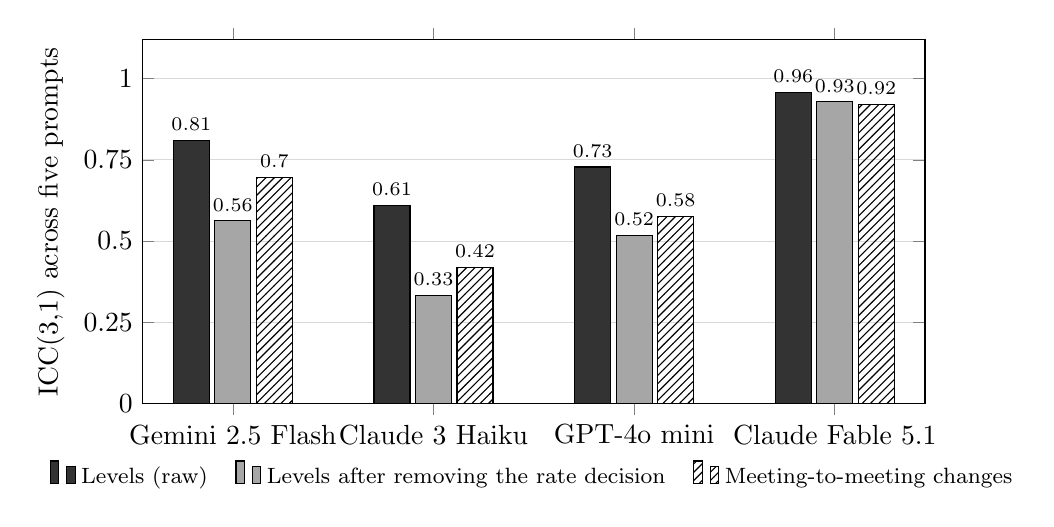
\begin{tikzpicture}
\begin{axis}[ybar, bar width=13pt, width=0.95\linewidth, height=6.2cm,
  ymin=0, ymax=1.12, ytick={0,0.25,0.5,0.75,1}, ylabel={ICC(3,1) across five prompts}, symbolic x coords={Gemini 2.5 Flash,Claude 3 Haiku,GPT-4o mini,Claude Fable 5.1},
  xtick=data, enlarge x limits=0.15, legend style={at={(0.5,-0.14)}, anchor=north, legend columns=-1, font=\footnotesize, draw=none, /tikz/every even column/.append style={column sep=8pt}},
  legend cell align=left, nodes near coords, nodes near coords style={font=\scriptsize, /pgf/number format/fixed, /pgf/number format/precision=2}, ymajorgrids, major grid style={black!15}]
\addplot[fill=black!80, draw=black] coordinates {(Gemini 2.5 Flash,0.810) (Claude 3 Haiku,0.609) (GPT-4o mini,0.728) (Claude Fable 5.1,0.957)};
\addlegendentry{Levels (raw)}
\addplot[fill=black!35, draw=black] coordinates {(Gemini 2.5 Flash,0.562) (Claude 3 Haiku,0.333) (GPT-4o mini,0.517) (Claude Fable 5.1,0.929)};
\addlegendentry{Levels after removing the rate decision}
\addplot[pattern=north east lines, draw=black] coordinates {(Gemini 2.5 Flash,0.697) (Claude 3 Haiku,0.419) (GPT-4o mini,0.577) (Claude Fable 5.1,0.920)};
\addlegendentry{Meeting-to-meeting changes}
\end{axis}
\end{tikzpicture}

\caption{Agreement across prompts by model, 2015--2019 block ($n=\R{icc.fable.n}$ statements). Part of
the inexpensive models' agreement on levels is agreement on the rate decision.}\label{fig:icc}
\end{figure}

The size of the drop depends on the sample. For Gemini it is \R{icc.gem.drop} in the 2015--2019 block but
\R{icc.gem04.drop} on 2004--2007 and \R{icc.gemfull.drop} on the full corpus. ICC is a ratio of
between-statement to total variance, so it is high when the statements in the sample differ a lot in
stance, as they do across the whole period from 2000 to 2026. Within a few years of similar statements,
prompt noise weighs more. The reliability of an LLM score is therefore a property of the model, the
prompt set and the sample together, and a researcher should report it for the sample actually used.

Fable's consistency is also high in a second sense: the \R{retest.n} cells it scored twice in separate
runs correlate at \R{retest.r}.

\subsection{Model choice versus prompt choice}

Prompt sensitivity is only one source of arbitrariness. A researcher also chooses a model. On the crossed
block I decompose the variance of the scores into statement, prompt and model effects and their
interactions, with a random-effects analysis of variance. With one score per cell, the three-way
interaction cannot be separated from noise, so it is part of the residual. Table~\ref{tab:variance}
reports the shares.

\begin{table}[t]
\centering
\caption{Variance decomposition: statement $\times$ prompt $\times$ model, 2015--2019 block}\label{tab:variance}
\small
% generated by paper/make_tables.py - do not edit
\begin{tabular}{@{}llr rrrrrrr@{}}
\toprule
Data & Scaling & $n$ & Statement & Prompt & Model & S$\times$P & S$\times$M & P$\times$M & Residual \\
\midrule
Levels & raw & 40 & 61.0 & 4.5 & 0.0 & 3.0 & 9.7 & 5.7 & 16.1 \\
Levels & std.\ within model & 40 & 61.3 & 4.6 & 0.0 & 3.0 & 9.2 & 6.0 & 15.9 \\
Changes & raw & 39 & 49.1 & 0.0 & 0.0 & 6.7 & 15.2 & 0.0 & 29.0 \\
Changes & std.\ within model & 39 & 50.2 & 0.0 & 0.0 & 6.4 & 15.2 & 0.0 & 28.3 \\
\bottomrule
\end{tabular}

\tabnote{\emph{Notes:} Shares of total variance (\%), random-effects ANOVA, \R{var.n} statements $\times$ 5
prompts $\times$ 4 models (Gemini 2.5 Flash, Claude 3 Haiku, GPT-4o mini, Claude Fable 5.1); negative
variance estimates are set to zero. ``Std.\ within model'' z-scores each model's scores first, which
removes scale differences between models. S$\times$P: prompts disagree about which statements are more
hawkish; S$\times$M: models disagree; the residual contains the three-way interaction and noise.}
\end{table}

On levels, agreed differences between statements account for \R{var.levels.raw.stmt} of the variance.
On changes, the agreed part falls to \R{var.changes.raw.stmt}. The main disagreement on changes is between
models: the statement-by-model interaction, which measures models disagreeing about which statements
became more hawkish, takes \R{var.changes.raw.sxm}, against \R{var.changes.raw.sxp} for the
statement-by-prompt interaction. The residual rises from \R{var.levels.raw.resid} on levels to
\R{var.changes.raw.resid} on changes. Standardising each model's scores first leaves these shares almost
unchanged, so they do not reflect differences in scale. For meeting-to-meeting changes, the choice of
model matters about twice as much as the choice of prompt. A robustness check across prompts alone
understates how much an LLM stance measure depends on the researcher's choices.

\subsection{Is the frontier model consistent because it recognises the text?}

One reading of Fable's high reliability is that it is simply a better reader. Another is that it
recognises each statement and recalls a fixed view of it, whatever the prompt
(Section~\ref{sec:recognition} shows it does recognise them). The two readings predict different
behaviour on statements the model has not seen. Fable's dating probe (Section~\ref{sec:cutoff}) suggests
that its knowledge fades from March 2026, so I scored the seven latest statements with all five prompts
and split them by whether the probe dated them exactly and with high confidence. The prompt spread (the standard deviation of the five scores) averages \R{spread.unknown}
on the \R{spread.unknown.n} statements it probably has not seen (March to July 2026) and \R{spread.known}
on the \R{spread.known.n} it dates confidently, against a median of \R{spread.pre.median} and a 90th
percentile of \R{spread.pre.p90} on the \R{spread.pre.n} pre-2024 statements with all prompts (Appendix
Table~\ref{tab:spread}). All seven recent statements lie between the \R{spread.pctmin} and
\R{spread.pctmax} quantiles of the pre-2024 spread, so Fable is somewhat less consistent on recent
statements than on old ones, whether it knows them or not. Two of the four statements it probably has
not seen are the unverified texts of June and July 2026 (Section~\ref{sec:data}); without them, the mean
spread of the remaining \R{spread.unknown.verified.n} is \R{spread.unknown.verified}, slightly above that
of the known statements. Statements this few cannot settle the question.

%=====================================================================================
\section{Recognition audit}\label{sec:recognition}

A model that recognises a statement could, in principle, score it with knowledge of what happened next:
the market reaction, the commentary, the following decisions. The standard response is to hide the
statement's identity before scoring. This section tests whether that works for FOMC statements. It asks
two questions: can Fable identify a blinded or paraphrased statement when asked, and does it identify
statements without being asked while it scores them?

\subsection{Dating on request}

Fable is shown each blinded pre-2024 statement and told that months, years, names and events have been
replaced by placeholders. It is asked to identify the meeting, to give its best guess even if unsure, and
to end with the year, the month and a confidence level (Appendix~\ref{app:prompts}). The probe covers all
\R{probe.blind.n} pre-2024 files, including \R{corpus.prenotices} notices. The exact month identifies the
meeting except in the \R{corpus.multimonth} months that have two statements. The same probe is
run on a sample of \R{probe.para.n} paraphrased statements spread evenly over the period, with a note that
the text may have been reworded.

A model with no memory can still date statements roughly. Policy-rate levels, purchase amounts and the
boilerplate of each era change slowly, so neighbouring statements look alike. To measure how far the
text alone goes, the text-similarity baseline represents each blinded statement by the frequencies of its
words and word pairs (TF-IDF weights), finds the most similar \emph{other} blinded statement by cosine
similarity, and takes that statement's date. The baseline is generous: it sees the true date of every
other statement. It can never name the exact meeting, because its answer is always another meeting, so I
count the statements whose two nearest neighbours are the meetings just before and just after. For
those, a reader who knew the sequence of statements could in principle infer the exact meeting. This
count is an upper bound for this method, not for every reader without memory: someone who knows the
history of the policy rate, the purchase programmes and the guidance dates could date many statements
more precisely without having read them before. The baseline shows how far textual similarity alone
goes.

\begin{table}[t]
\centering
\caption{Dating blinded and paraphrased statements}\label{tab:dating}
\footnotesize
\setlength{\tabcolsep}{4pt}
% generated by paper/make_tables.py - do not edit
\begin{tabular}{@{}l cccc@{}}
\toprule
 & \multicolumn{3}{c}{Claude Fable 5.1, asked for the date} & Text-similarity \\
\cmidrule(lr){2-4}
 & Blinded & Paraphrased & Blinded & baseline \\
 & 2000--2023 & 2000--2023 (sample) & 2024--2026 & 2000--2023 \\
\midrule
Exact meeting & 202/206 (98.1\%) & 28/30 (93.3\%) & 19/22 (86.4\%) & $\le$ 89/206 (43.2\%)$^a$ \\
Within 1 month & 204/206 (99.0\%) & 29/30 (96.7\%) & 21/22 (95.5\%) & 106/206 (51.5\%) \\
Within 3 months & 206/206 (100.0\%) & 30/30 (100.0\%) & 22/22 (100.0\%) & 190/206 (92.2\%) \\
\addlinespace
ZLB statements, exact & 55/56 (98.2\%) & 6/8 (75.0\%) & -- & $\le$ 28/56 (50.0\%)$^a$ \\
Confidence ``high'' & 205/206 (99.5\%) & 29/30 (96.7\%) & 17/22 (77.3\%) & -- \\
\bottomrule
\end{tabular}

\tabnote{\emph{Notes:} Fable is asked for the year and month of the meeting. Paraphrased = an evenly
spaced sample of \R{probe.para.n} paraphrased statements. 2024--2026 = all blinded statements from 2024 on.
ZLB (zero-lower-bound) statements: January 2009 to October 2015, when the target range was the same at every
meeting (\R{corpus.zlbnotices} of them a notice). The 2000--2023 columns include \R{corpus.prenotices}
notices. Text-similarity baseline: each blinded statement takes the date of its most similar other
blinded statement (TF-IDF over words and word pairs, cosine). $^a$Statements whose two nearest neighbours
are the meetings just before and after, an upper bound on exact recovery for this method.}
\end{table}

\begin{figure}[t]
\centering
% generated by paper/make_tables.py
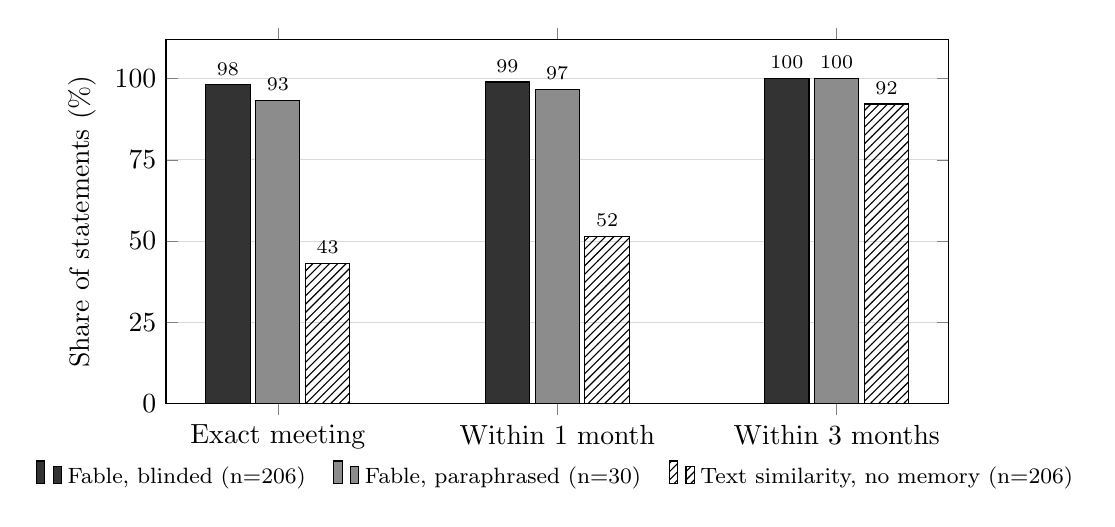
\begin{tikzpicture}
\begin{axis}[ybar, bar width=16pt, width=0.95\linewidth, height=6.2cm,
  ymin=0, ymax=112, ytick={0,25,50,75,100}, ylabel={Share of statements (\%)}, symbolic x coords={Exact meeting,Within 1 month,Within 3 months},
  xtick=data, enlarge x limits=0.2, legend style={at={(0.5,-0.14)}, anchor=north, legend columns=-1, font=\footnotesize, draw=none, /tikz/every even column/.append style={column sep=8pt}},
  legend cell align=left, nodes near coords, nodes near coords style={font=\scriptsize, /pgf/number format/fixed, /pgf/number format/precision=0}, ymajorgrids, major grid style={black!15}]
\addplot[fill=black!80, draw=black] coordinates {(Exact meeting,98.1) (Within 1 month,99.0) (Within 3 months,100.0)};
\addlegendentry{Fable, blinded (n=206)}
\addplot[fill=black!45, draw=black] coordinates {(Exact meeting,93.3) (Within 1 month,96.7) (Within 3 months,100.0)};
\addlegendentry{Fable, paraphrased (n=30)}
\addplot[pattern=north east lines, draw=black] coordinates {(Exact meeting,43.2) (Within 1 month,51.5) (Within 3 months,92.2)};
\addlegendentry{Text similarity, no memory (n=206)}
\end{axis}
\end{tikzpicture}

\caption{Dating accuracy. Fable on blinded and paraphrased statements against a text-similarity baseline
that has no memory. For the baseline, ``exact meeting'' is the upper bound described in the text.}\label{fig:dating}
\end{figure}

Table~\ref{tab:dating} and Figure~\ref{fig:dating} show the results. Fable names the exact month of
\R{probe.blind.exact} of the \R{probe.blind.n} blinded statements (\R{probe.blind.exactpct}) and places
every one within three months. The four misses (\R{probe.blind.misses}) are each an adjacent meeting. On
the zero-lower-bound statements, where the rate level gives no clue, it is exact on \R{probe.blind.zlb} of
\R{probe.blind.zlbn}. It reports high confidence on \R{probe.blind.high} statements. Its replies also
restore details that blinding removed: for the blinded statement of 18 December 2013 it names Eric
Rosengren as the dissenter, and for 25 June 2003 it says that Robert Parry dissented in favour of a larger
cut. Both are correct. Paraphrasing barely helps: Fable names the exact month of \R{probe.para.exact} of
the \R{probe.para.n} paraphrased statements.

The baseline shows what the text alone can do. It places \R{base.w3pct} of the statements within three
months and \R{base.w1pct} within one month, so dating to within a few months is not evidence of memory.
Exact identification is more telling. The baseline's upper bound on exact recovery is \R{base.brpct}
(\R{base.br} of \R{base.n}), and \R{base.zlb.br} of \R{probe.blind.zlbn} at the zero lower bound, against
Fable's \R{probe.blind.exactpct} and \R{probe.blind.zlb} of \R{probe.blind.zlbn}. The probe therefore shows
that Fable has knowledge sufficient to identify the individual meeting. Whether that knowledge is of the
statements themselves or of a detailed policy history cannot be separated here, but the
zero-lower-bound statements, which share a rate level and differ mainly in purchase amounts and wording,
are the hardest case for general knowledge, and the restored dissenters' names point to the statements
themselves.

\subsection{Recognition while scoring}

Dating on request shows that Fable \emph{can} identify the statements. A more direct question is whether
it does so when it is only asked for a score. I search every stored scoring reply for a date in the form
``$\langle$month$\rangle$ [day,] $\langle$year$\rangle$'' or ``$\langle$year$\rangle$
statement/meeting/decision'' and check whether it is the statement's own month and year. On blinded and
paraphrased text no date is in the input, so a correct date came from the model. On the original text of
the five-prompt runs, \R{nav.n} early statements contained their year in a navigation line
(Section~\ref{sec:data}), but not the month. The counts are lower bounds: most prompts ask for the number
only, and replies were stored cut at 300 characters.

\begin{table}[t]
\centering
\caption{Scoring replies that name the statement's date, unprompted}\label{tab:spontaneous}
\footnotesize
\setlength{\tabcolsep}{4pt}
% generated by paper/make_tables.py - do not edit
\begin{tabular}{@{}lll rrr@{}}
\toprule
Scores & Text & Prompt & Replies & Name a date & Own month and year \\
\midrule
Claude Fable 5.1, five prompts & original & all & 1228 & 245 (20.0\%) & 241 (19.6\%) \\
\addlinespace[2pt]
 &  & P1\_minimal & 255 & 21 (8.2\%) & 21 (8.2\%) \\
 &  & P2\_defined & 244 & 43 (17.6\%) & 43 (17.6\%) \\
 &  & P3\_analyst & 242 & 2 (0.8\%) & 2 (0.8\%) \\
 &  & P4\_reversed & 244 & 32 (13.1\%) & 32 (13.1\%) \\
 &  & P5\_reason\_first & 243 & 147 (60.5\%) & 143 (58.8\%) \\
\addlinespace
Claude Fable 5.1, P1 re-run & original & all & 206 & 20 (9.7\%) & 20 (9.7\%) \\
\addlinespace
Claude Fable 5.1, P1 & blinded & all & 206 & 23 (11.2\%) & 23 (11.2\%) \\
\addlinespace
Claude Fable 5.1, P1 & paraphrased & all & 206 & 7 (3.4\%) & 7 (3.4\%) \\
\addlinespace
Gemini 2.5 Flash, five prompts & original & all & 1140 & 0 (0.0\%) & 0 (0.0\%) \\
\addlinespace
GPT-4, P1 & original & all & 228 & 0 (0.0\%) & 0 (0.0\%) \\
\bottomrule
\end{tabular}

\tabnote{\emph{Notes:} A reply ``names a date'' if it contains ``$\langle$month$\rangle$ [day,]
$\langle$year$\rangle$'' or ``$\langle$year$\rangle$ statement/meeting/decision''. ``Own month and year'':
the named date is the statement's own. Replies stored before 3 October 2026 were cut at 300 characters,
so the shares are lower bounds. The five-prompt Fable file includes repeat runs of some cells.}
\end{table}

Table~\ref{tab:spontaneous} reports the counts. Across its five-prompt runs on the original text, Fable
names the statement's own month and year in \R{spont.scoresfable.all.pct} of its replies. The share
depends on whether the prompt lets it talk: \R{spont.scoresfable.p5.pct} for the reason-first prompt P5,
\R{spont.scoresfable.p3.pct} for the analyst prompt P3. On blinded text, with P1, it does so in
\R{spont.blindfable.all.pct} of replies, slightly more than the \R{spont.cleanfable.all.pct} of the same
prompt on the cleaned original. On paraphrased text the share falls to \R{spont.parafable.all.pct}.
Gemini never names a date in \R{spont.fullgemini.all.n} replies, nor does GPT-4 in
\R{spont.gpt4p1.all.n}.

\begin{table}[t]
\centering
\caption{Excerpts from Fable's scoring replies}\label{tab:quotes}
\footnotesize
% generated by paper/make_tables.py - do not edit
\begin{tabular}{@{}llp{10.2cm}@{}}
\toprule
Statement & Prompt & Excerpt of the scoring reply \\
\midrule
2013-10-30 (blinded) & P1\_minimal & \ldots{}This is the October 2013 FOMC statement: continued QE at \$85B/mo\ldots \\
2014-01-29 (blinded) & P1\_minimal & \ldots{}This is the January 2014 FOMC statement: a second measured taper\ldots \\
2000-12-19 (original) & P4\_reversed & \ldots{}inflation to economic weakness --- a clear dovish pivot signaling upcoming cuts (which came in January 2001)\ldots \\
2004-05-04 (original) & P2\_defined & \ldots{}removed at a pace that is likely to be measured'' --- a clear hawkish shift setting up the June 2004 hike,\ldots \\
2007-12-11 (original) & P5\_reason\_first & \ldots{}acknowledged intensifying housing correction and rising financial strains (markets had hoped for more)\ldots \\
2016-03-16 (original) & P1\_minimal & \ldots{}dissent (George). Overall mildly dovish relative to prior expectations (dot plot cut from 4 to 2 hikes)\ldots \\
2016-11-02 (original) & P5\_reason\_first & \ldots{}continued to strengthen'' --- explicit signal that a hike is approaching (widely read as teeing up December)\ldots \\
\bottomrule
\end{tabular}

\tabnote{\emph{Notes:} Verbatim excerpts from stored scoring replies (the blinded ones from P1 on blinded
text). Each was asked only for a stance score. Several cite information that was not in the statement:
later decisions, the market's reaction or commentary, or the projections released with it.}
\end{table}

Table~\ref{tab:quotes} gives examples. Some replies go beyond naming the meeting and bring in information
that was not in the statement: later decisions (cuts ``came in January 2001''; a statement was ``setting
up the June 2004 hike''), the market's reaction and later commentary (``markets had hoped for more'';
``widely read as teeing up December''), and the projections released alongside the statement (the
``dot plot cut from 4 to 2 hikes''). This is direct evidence that the model retrieves knowledge from
outside the text, including knowledge of later events, while it scores. It does not show that this knowledge moves
the score, but it shows that the scores cannot be assumed to come from the text alone.

\subsection{What recognition implies}

The same excerpts show a second habit: Fable often judges a statement relative to the previous one or
to what markets expected (``mildly dovish relative to prior expectations''). A score formed against
expectations is closer to a policy surprise than a reading of the text in isolation would be, and knowing
the expectations at each meeting is itself a form of recognition.

Recognition is necessary for a model to recall a statement's market reaction, but it is not evidence that
the model does so. The finding is therefore not that Fable's scores are contaminated. It is that the
tools meant to rule contamination out do not work on this corpus. Blinding and paraphrasing were meant to
create an unrecognised version of each statement, so that scores on recognised and unrecognised text
could be compared. With \R{probe.hold.recog} of the \R{probe.hold.n} probed hold meetings dated exactly,
there is no unrecognised group to compare with.

This finding complements \citet{glasserman2023}, who remove company names from news headlines to limit
look-ahead bias. Headlines about individual firms are many, short and mostly obscure. FOMC statements are
few, long, and widely read and discussed; their content identifies them. For documents like these,
anonymisation and paraphrase do not rule out look-ahead bias. Only models whose training data stop before the documents
\citep{he2025,drinkall2024}, or documents the model cannot have seen, can do that.

\subsection{Where Fable's knowledge ends}\label{sec:cutoff}

Running the same probe on the \R{probe.post.n} blinded statements from 2024 to 2026 locates the end of
Fable's knowledge (Appendix Table~\ref{tab:lateprobe}). It dates \R{probe.post.exact} of them exactly,
including every statement from the second half of 2024 and from 2025, all with high confidence. Its
confidence falls in 2026: of the four statements from the first half of 2026 it dates only one with high
confidence, and it misses July 2026. Its knowledge therefore extends to about early 2026. The 2024--2025
statements, often treated as a ``post-cutoff'' test sample, are not unseen for this model.

%=====================================================================================
\section{Validity: do score changes track market surprises?}\label{sec:validity}

\subsection{Specification}

If a stance score measures what the statement says about future policy, changes in the score should move
with the market's reading of the announcement. I estimate
\begin{equation}
y_t = \alpha + \beta\,\text{dScore}_t + \varepsilon_t
\end{equation}
over statements up to December 2023, where $y_t$ is a market outcome at statement $t$. Standard errors
are Newey--West \citep{newey1987} with a Bartlett kernel and $\lfloor 4(n/100)^{2/9}\rfloor$ lags, a common
rule of thumb associated with \citet{newey1994}, which is \R{prim.lag} meetings in these samples;
$p$-values use the Student $t$ distribution.

The \emph{primary specification} uses MPS as the outcome, Fable's dScore, the policy corpus and hold
meetings only, with no controls. Hold meetings are the natural test: at a rate change both the score and
the surprise move with the decision, so their correlation could simply reflect the decision, which no
LLM is needed to read. MPS is measured in a 30-minute window and so isolates the announcement.

This specification was frozen on 3 October 2026, after earlier versions had been estimated and seen. The
choice of hold meetings, of MPS as the outcome, of the five-prompt consensus over a single prompt, of
whether to control for the rate change, and of the corpus definition were all made after looking at
results. The corpus definition, in particular, followed an independent review of the code which found
that seven non-policy notices, then coded as hold meetings, drove the earlier daily-yield results. The
adjusted $p$-values below correct for the twelve regressions in Fable's primary family. They do not
correct for this search, so even they overstate the evidence. The main analysis run reports
\R{regs.csv} regression coefficients with their tests (Appendix~\ref{app:disclose}), and the checks in
this section add more.

\subsection{The primary result}

\begin{table}[t]
\centering
\caption{The primary specification and its family}\label{tab:primary}
\small
% generated by paper/make_tables.py - do not edit
\begin{tabular}{@{}lll rrrr rr@{}}
\toprule
Outcome & Meetings & Control & $n$ & $\hat\beta$ & NW $t$ & $p$ & Holm $p$ & Bonferroni $p$ \\
\midrule
MPS & all & -- & 198 & 0.049 & 3.02 & 0.003 & 0.034 & 0.034 \\
\textbf{MPS} & \textbf{hold} & \textbf{--} & \textbf{132} & \textbf{0.033} & \textbf{2.39} & \textbf{0.018} & \textbf{0.199} & \textbf{0.217} \\
MPS & all & change\_bp & 198 & 0.036 & 2.27 & 0.025 & 0.245 & 0.294 \\
$d_{10}$ (bp) & hold & -- & 120 & 5.20 & 1.74 & 0.084 & 0.756 & 1.000 \\
$d_{10}$ (bp) & all & change\_bp & 173 & 4.39 & 1.52 & 0.130 & 1.000 & 1.000 \\
$d_{10}$ (bp) & all & -- & 173 & 4.27 & 1.44 & 0.151 & 1.000 & 1.000 \\
$d_2$ (bp) & all & change\_bp & 173 & 4.93 & 1.41 & 0.160 & 1.000 & 1.000 \\
$d_2$ (bp) & all & -- & 173 & 5.02 & 1.41 & 0.162 & 1.000 & 1.000 \\
$d_2$ (bp) & hold & -- & 120 & 3.77 & 1.03 & 0.306 & 1.000 & 1.000 \\
MPS\_ORTH & all & -- & 189 & 0.014 & 0.79 & 0.431 & 1.000 & 1.000 \\
MPS\_ORTH & hold & -- & 125 & 0.011 & 0.69 & 0.490 & 1.000 & 1.000 \\
MPS\_ORTH & all & change\_bp & 189 & 0.010 & 0.56 & 0.578 & 1.000 & 1.000 \\
\midrule
MPS, 2003+ sample & hold & -- & 120 & 0.038 & 2.65 & 0.009 & -- & -- \\
\bottomrule
\end{tabular}

\tabnote{\emph{Notes:} Fable consensus dScore, policy corpus, statements to December 2023. Each row is one
regression of the outcome on dScore (and the rate change in basis points, where shown). The family is
the twelve combinations of four outcomes (MPS, MPS\_ORTH, $d_2$, $d_{10}$) and three samples; Holm and
Bonferroni adjust for these twelve tests only. Newey--West $t$ with \R{prim.lag} lags. The primary
specification is in bold. The last row repeats it on the 2003+ meetings that also have daily yields.}
\end{table}

Table~\ref{tab:primary} reports the primary regression and its family. On \R{prim.n} hold meetings from
\R{prim.first} to \R{prim.last}, the slope is \R{prim.beta} percentage points of MPS per unit of dScore,
with a Newey--West $t$ of \R{prim.t} ($p=\R{prim.p}$) and an $R^2$ of \R{prim.r2}. The OLS and
heteroskedasticity-robust $t$-statistics are similar (\R{prim.tols} and \R{prim.thc}). In economic terms
the relation is small: a one-standard-deviation change in dScore (\R{fable.sd}) goes with
\R{prim.persd} percentage points of MPS, about \R{prim.persd.ratio} of the standard deviation of MPS at
hold meetings. On the \R{prim03.n} hold meetings from 2003 onwards, which also have daily yields, the
$t$-statistic is \R{prim03.t}.

The result does not survive a correction for multiple testing. Its Holm-adjusted $p$-value
\citep{holm1979} over the twelve tests is \R{fam.MPS.hold.none.holm} (Bonferroni
\R{fam.MPS.hold.none.bonf}). The only regression in the family that survives is MPS on all meetings
($t=\R{fam.MPS.all.none.t}$, Holm $p=\R{fam.MPS.all.none.holm}$). That regression includes the rate
decisions; controlling for the size of the rate change lowers its $t$ to \R{fam.MPS.all.ctrl.t}.

\subsection{Other outcomes and other scores}

\begin{table}[t]
\centering
\caption{Hold meetings: slopes on dScore by outcome and score}\label{tab:secondary}
\footnotesize
\setlength{\tabcolsep}{4.5pt}
% generated by paper/make_tables.py - do not edit
\begin{tabular}{@{}l r ccccccc@{}}
\toprule
Outcome & $n$ & Fable & Gemini & Dictionary & Fable P1 & P1 blinded & P1 paraphr. & GPT-4 P1 \\
\midrule
MPS & 132 & 0.033 & 0.003 & $-$0.010 & 0.026 & 0.017 & 0.014 & $-$0.006 \\
 & & (2.39) & (0.27) & ($-$0.99) & (2.20) & (1.43) & (0.90) & ($-$0.63) \\
\addlinespace[3pt]
MPS\_ORTH & 125 & 0.011 & $-$0.009 & $-$0.021 & 0.008 & $-$0.001 & $-$0.009 & $-$0.016 \\
 & & (0.69) & ($-$0.91) & ($-$1.75) & (0.55) & ($-$0.06) & ($-$0.53) & ($-$1.92) \\
\addlinespace[3pt]
$t_2$ (30-min, bp) & 132 & 3.76 & 0.03 & $-$1.52 & 2.66 & 1.72 & 1.42 & $-$1.11 \\
 & & (2.05) & (0.03) & ($-$1.39) & (1.74) & (1.12) & (0.74) & ($-$1.03) \\
\addlinespace[3pt]
$t_{10}$ (30-min, bp) & 132 & 2.98 & 0.06 & $-$0.54 & 1.85 & 1.45 & 0.96 & $-$0.61 \\
 & & (2.10) & (0.10) & ($-$0.66) & (1.75) & (1.38) & (0.68) & ($-$0.94) \\
\addlinespace[3pt]
$d_2$ (daily, bp) & 120 & 3.77 & $-$2.26 & $-$0.36 & 2.21 & 0.06 & $-$0.97 & $-$2.55 \\
 & & (1.03) & ($-$1.29) & ($-$0.17) & (0.74) & (0.02) & ($-$0.26) & ($-$1.88) \\
\addlinespace[3pt]
$d_{10}$ (daily, bp) & 120 & 5.20 & $-$0.15 & 1.70 & 3.18 & 1.44 & 1.10 & $-$0.05 \\
 & & (1.74) & ($-$0.11) & (0.87) & (1.40) & (0.61) & (0.37) & ($-$0.04) \\
\bottomrule
\end{tabular}

\tabnote{\emph{Notes:} Slope of each outcome on dScore with Newey--West $t$ in parentheses; hold meetings,
policy corpus, statements to December 2023. Fable and Gemini: five-prompt consensus with prompt fixed
effects. Dictionary: word-count score. Fable P1: re-score with prompt P1 on the cleaned original text; P1
blinded and P1 paraphrased: the same prompt on the blinded and paraphrased versions. GPT-4: prompt P1;
it lacks a few statements, so its $n$ is up to three lower. MPS in percentage points per unit of dScore,
yields in basis points.}
\end{table}

Table~\ref{tab:secondary} reports every outcome for every score on hold meetings. Three facts stand out.

First, Fable's dScore is unrelated to MPS\_ORTH ($t=\R{hold.fable.MPS_ORTH.t}$), the part of the surprise
that \citet{bauer2023reassessment} show is not predictable from macroeconomic and financial data released
before the meeting. Its relation is with the predictable part: on the same \R{extra.predpart.n} meetings,
regressing MPS minus MPS\_ORTH on dScore gives $t=\R{extra.predpart.t}$ (Table~\ref{tab:extra}; an
exploratory check). A model that knows the economic context of each meeting would pick up exactly that
component, whether it reads it from the text or recalls it.

Second, the 30-minute yield changes give $t$-statistics of \R{hold.fable.t2.t} ($t_2$) and
\R{hold.fable.t10.t} ($t_{10}$), close to the MPS result. They are not independent evidence: on hold
meetings their correlation with MPS is \R{desc.corr.MPS.t2} and \R{desc.corr.MPS.t10}. The daily yield
changes are not significantly related to dScore ($t$ of \R{hold.fable.d2.t} for $d_2$ and
\R{hold.fable.d10.t} for $d_{10}$). Daily changes also contain the day's other news, so they are a noisier
outcome.

Third, no other score shows a relation. Gemini's dScore has $t$-statistics between
\R{hold.gemini.d2.t} and \R{hold.gemini.MPS.t} on the six outcomes, the dictionary's are of either sign
and none is significant, and GPT-4's are all negative or near zero. Fable's own single-prompt re-score on
the cleaned text gives an MPS $t$ of \R{hold.clean.MPS.t}; on blinded and paraphrased text the same
prompt gives \R{hold.blind.MPS.t} and \R{hold.para.MPS.t} (Section~\ref{sec:versions-validity}).

\subsection{Robustness}\label{sec:robust}

\begin{table}[t]
\centering
\caption{Hold-meeting $t$-statistics under other score constructions and corpora}\label{tab:variants}
\footnotesize
\setlength{\tabcolsep}{4pt}
% generated by paper/make_tables.py - do not edit
\begin{tabular}{@{}l rrrrrrrrrr@{}}
\toprule
 & \multicolumn{2}{c}{MPS} & \multicolumn{2}{c}{$t_{2}$} & \multicolumn{2}{c}{$t_{10}$} & \multicolumn{2}{c}{$d_{2}$} & \multicolumn{2}{c}{$d_{10}$} \\
\cmidrule(lr){2-3}\cmidrule(lr){4-5}\cmidrule(lr){6-7}\cmidrule(lr){8-9}\cmidrule(lr){10-11}
Variant & $n$ & $t$ & $n$ & $t$ & $n$ & $t$ & $n$ & $t$ & $n$ & $t$ \\
\midrule
Default: policy corpus, prompt-demeaned consensus & 132 & 2.39 & 132 & 2.05 & 132 & 2.10 & 120 & 1.03 & 120 & 1.74 \\
Strict corpus (also drops 2007-08-17, 2020-03-23) & 130 & 2.18 & 130 & 2.11 & 130 & 2.48 & 118 & 1.98 & 118 & 2.73 \\
All files (the seven notices kept) & 137 & 2.33 & 137 & 2.23 & 137 & 2.59 & 126 & 2.32 & 126 & 2.76 \\
Consensus over prompts common to both statements & 130 & 2.36 & 130 & 2.02 & 130 & 2.07 & 118 & 1.00 & 118 & 1.65 \\
Raw consensus (no prompt fixed effects) & 132 & 2.38 & 132 & 2.04 & 132 & 2.09 & 120 & 1.01 & 120 & 1.73 \\
One prompt only (P1\_minimal) & 117 & 2.20 & 117 & 1.84 & 117 & 1.96 & 105 & 0.41 & 105 & 1.27 \\
\bottomrule
\end{tabular}

\tabnote{\emph{Notes:} Fable dScore, hold meetings, statements to December 2023, Newey--West $t$. Strict
corpus: policy corpus without the two unscheduled policy statements (17 August 2007 and 23 March 2020).
All files: also keeps the seven notices. Matched: each pair's change is averaged over the prompts scored
at both statements. Raw: mean over available prompts without prompt fixed effects. P1: prompt P1 only.}
\end{table}

\paragraph{Score construction and corpus.} Table~\ref{tab:variants} re-estimates the hold-meeting
regressions under five alternatives. The MPS $t$-statistic stays between \R{var.strict.MPS.t} and
\R{var.default.MPS.t} in every variant, including the single prompt P1 (\R{var.p1.MPS.t}). The daily
yields do not behave this way. Under the policy corpus their $t$-statistics are \R{var.default.d2.t}
($d_2$) and \R{var.default.d10.t} ($d_{10}$). Dropping the two unscheduled policy statements raises them to
\R{var.strict.d2.t} and \R{var.strict.d10.t}, and keeping the non-policy notices gives
\R{var.all.d2.t} and \R{var.all.d10.t}. A result that moves by one unit of $t$ depending on whether two
statements are in the sample cannot be called established, whichever corpus one prefers. The policy
corpus was chosen before the strict variant was run. The all-files corpus is not a defensible
alternative: it treats liquidity and swap-line notices as hold meetings and measures the next
statement's dScore against them.

\begin{table}[t]
\centering
\caption{Placebo days for the daily yield regressions}\label{tab:placebo}
\small
% generated by paper/make_tables.py - do not edit
\begin{tabular}{@{}ll rrrrrr@{}}
\toprule
Corpus & Outcome & Actual $t$ & Placebo days & $|t|>1.96$ & $|t|\ge$ actual & 95th pct.\ $|t|$ & Max $|t|$ \\
\midrule
Policy (default) & $d_{2}$ & 1.03 & 60 & 7 & 27 & 2.37 & 2.71 \\
 & $d_{10}$ & 1.74 & 60 & 9 & 15 & 2.64 & 3.50 \\
Strict & $d_{2}$ & 1.98 & 60 & 6 & 6 & 2.07 & 2.35 \\
 & $d_{10}$ & 2.73 & 60 & 6 & 2 & 2.44 & 3.05 \\
All files & $d_{2}$ & 2.32 & 60 & 4 & 1 & 2.01 & 2.39 \\
 & $d_{10}$ & 2.76 & 60 & 10 & 3 & 2.57 & 3.19 \\
\bottomrule
\end{tabular}

\tabnote{\emph{Notes:} Fable dScore, hold meetings. Each placebo replaces the statement-day yield change
with the change $k$ trading days earlier or later ($k=\pm1,\ldots,\pm30$) and re-runs the regression.
Columns give the number of placebo days whose $|t|$ exceeds 1.96 and the actual $t$, and the 95th
percentile and maximum of the 60 placebo $|t|$ values.}
\end{table}

\paragraph{Placebo days.} If the daily yield regressions had well-behaved $t$-statistics, the same
regression on yield changes from days without a statement should rarely give $|t|>1.96$. Table~\ref{tab:placebo}
shows that it often does. Under the policy corpus, \R{placebo.d10.over196} of 60 placebo days give
$|t|>1.96$ for $d_{10}$, the 95th percentile of placebo $|t|$ is \R{placebo.d10.p95}, and
\R{placebo.d10.overreal} placebo days match or exceed the actual \R{placebo.d10.real}. The actual
$t$-statistics are ordinary draws from this distribution. In the other two corpora the picture is
different: the actual $d_{10}$ $t$ is matched by only \R{placebo.strict.d10.overreal} of 60 placebo days
under the strict corpus and \R{placebo.all.d10.overreal} under the all-files corpus, and the actual $d_2$
$t$ by \R{placebo.strict.d2.overreal} and \R{placebo.all.d2.overreal}. That is the strongest evidence for a
daily yield link in this paper. It appears only in corpora that differ from the policy corpus by two
borderline statements, or that keep the non-policy notices. The fat tails of the placebo distributions
are a warning in their own right: GPT-4's coarse score gives a $t$ of \R{h.gpt4.d2.hold-pre.t} for $d_2$
before its cutoff (Section~\ref{sec:cannot}), with the wrong sign, which shows how large a spurious
daily-yield $t$ can be here.

\paragraph{Influence.} Table~\ref{tab:influence} and Figure~\ref{fig:scatter} show how much the MPS result
depends on a few meetings. Leaving out one meeting at a time gives $t$-statistics between
\R{infl.MPS.loomin} and \R{infl.MPS.loomax}. Dropping the five most influential meetings one after
another gives \R{infl.MPS.path}. This greedy drop removes the observations most favourable to the result,
so it weakens any effect of this size. To calibrate it, I simulate 200 data sets from the fitted line with
resampled residuals, so that the true slope equals the estimate, and apply the same drop. The median
$t$-statistic falls from \R{bench.full} to \R{bench.after}, and \R{bench.sharepct} of the simulations end
at or below the actual \R{infl.MPS.after5}. The influence analysis is therefore what a real effect of
this size would produce, and it is not evidence against the result. The relation is also not driven by
outliers: winsorising both variables at the 2.5th and 97.5th percentiles gives $t=\R{extra.winsor.t}$,
the Spearman rank correlation is \R{prim.spearman}, and a permutation test that shuffles dScore across
hold meetings gives $p=\R{prim.perm}$ (which, like the other $p$-values, ignores the specification
search).

The most influential meeting for every outcome is the statement of 13 December 2023, widely read as
signalling the end of the hiking cycle. Among the others are the statement of 28 January 2004, which
replaced the promise to keep rates low for a ``considerable period'' with a promise to be ``patient'', and
that of 28 October 2015, which pointed to a possible hike at the next meeting. These meetings are not
recognised more often than others: Fable names their month and year unprompted in \R{name.infl} scoring
replies (\R{name.inflpct}), against \R{name.other} (\R{name.otherpct}) at the other hold meetings.
Conversely, Fable's dScore misses the two largest asset-purchase surprises among the hold meetings: it is
\R{lsap.2009-03-18.ds} for 18 March 2009, when the 10-year yield changed by \R{lsap.2009-03-18.d10} basis
points in a day, and \R{lsap.2013-09-18.ds} for 18 September 2013 (\R{lsap.2013-09-18.d10} basis points).

\begin{table}[t]
\centering
\caption{Influence of individual meetings}\label{tab:influence}
\footnotesize
% generated by paper/make_tables.py - do not edit
\begin{tabular}{@{}l rrr l@{}}
\toprule
Outcome & Full $t$ & LOO min & LOO max & $t$ after dropping 1, 2, \ldots, 5 meetings (greedy) \\
\midrule
MPS & 2.39 & 2.13 & 3.08 & 2.13 $\to$ 1.87 $\to$ 1.58 $\to$ 1.34 $\to$ 1.12 \\
 & \multicolumn{4}{l}{\footnotesize dropped in order: 2023-12-13, 2007-08-17, 2002-08-13, 2004-01-28, 2015-10-28} \\
$d_{2}$ & 1.03 & 0.64 & 1.99 & 0.64 $\to$ 0.40 $\to$ 0.14 $\to$ $-$0.09 $\to$ $-$0.30 \\
 & \multicolumn{4}{l}{\footnotesize dropped in order: 2023-12-13, 2015-10-28, 2004-01-28, 2015-09-17, 2019-06-19} \\
$d_{10}$ & 1.74 & 1.54 & 2.74 & 1.54 $\to$ 1.38 $\to$ 1.21 $\to$ 1.03 $\to$ 0.85 \\
 & \multicolumn{4}{l}{\footnotesize dropped in order: 2023-12-13, 2015-10-28, 2013-06-19, 2011-08-09, 2015-09-17} \\
$t_{2}$ & 2.05 & 1.79 & 2.60 & 1.79 $\to$ 1.57 $\to$ 1.36 $\to$ 1.13 $\to$ 0.91 \\
 & \multicolumn{4}{l}{\footnotesize dropped in order: 2023-12-13, 2015-10-28, 2004-01-28, 2019-01-30, 2002-08-13} \\
$t_{10}$ & 2.10 & 1.90 & 2.48 & 1.90 $\to$ 1.73 $\to$ 1.58 $\to$ 1.43 $\to$ 1.28 \\
 & \multicolumn{4}{l}{\footnotesize dropped in order: 2023-12-13, 2015-10-28, 2019-01-30, 2004-01-28, 2013-06-19} \\
\bottomrule
\end{tabular}

\tabnote{\emph{Notes:} Fable dScore, hold meetings, policy corpus, Newey--West $t$. LOO: range of $t$ when
one meeting is left out. Greedy: at each step the meeting whose removal lowers $t$ most is dropped.}
\end{table}

\begin{figure}[t]
\centering
% generated by paper/make_tables.py
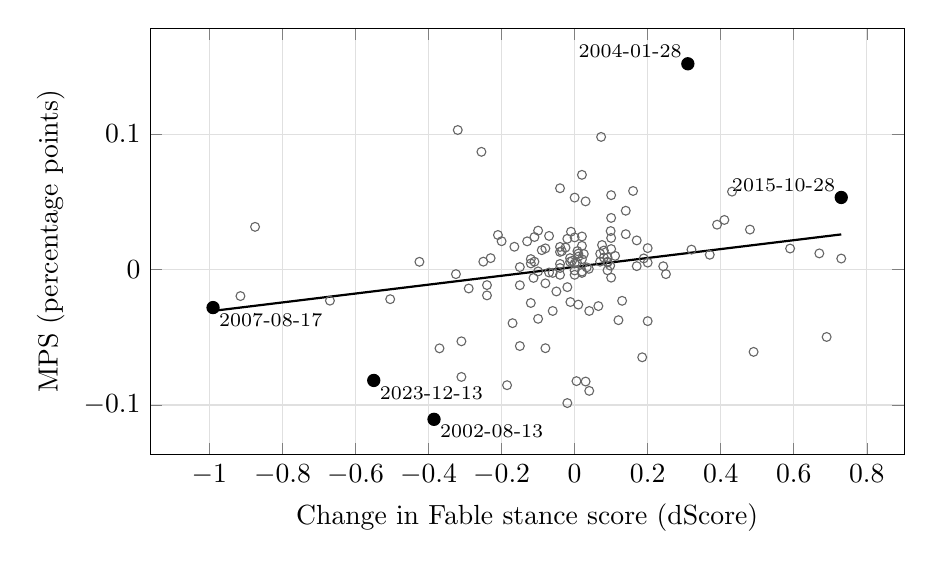
\begin{tikzpicture}
\begin{axis}[width=0.92\linewidth, height=7cm, xlabel={Change in Fable stance score (dScore)},
  ylabel={MPS (percentage points)}, ymajorgrids, xmajorgrids, major grid style={black!12}, clip=false]
\addplot[only marks, mark=o, mark size=1.6pt, black!60] coordinates {(-0.5050,-0.0219) (0.0000,0.0237) (0.0000,0.0531) (-0.0900,0.0143) (-0.8750,0.0315) (0.4100,0.0366) (0.4900,-0.0608) (-0.1000,-0.0364) (-0.2000,0.0209) (-0.0400,-0.0039) (0.4800,0.0295) (-0.0400,0.0600) (-0.1200,0.0077) (-0.1850,-0.0854) (0.0400,-0.0306) (0.0000,0.0044) (0.0300,-0.0827) (0.1400,0.0434) (-0.1500,-0.0565) (0.7300,0.0081) (-0.1200,-0.0247) (-0.0100,0.0279) (0.0200,-0.0015) (0.0100,-0.0259) (0.0000,-0.0007) (0.0400,-0.0896) (0.0300,0.0503) (0.0200,0.0244) (-0.0800,-0.0102) (0.6900,-0.0498) (-0.2400,-0.0191) (-0.3200,0.1030) (0.0900,-0.0006) (-0.0800,-0.0581) (0.1400,0.0261) (0.1000,0.0549) (0.1000,-0.0060) (-0.0200,-0.0986) (-0.0200,-0.0130) (0.1000,0.0151) (0.1000,0.0381) (-0.0600,-0.0306) (-0.0400,0.0011) (-0.0800,0.0156) (-0.0500,-0.0162) (-0.0700,-0.0022) (-0.1100,0.0058) (0.0900,0.0052) (0.0200,-0.0025) (0.2000,0.0158) (-0.0600,-0.0025) (0.0800,0.0140) (-0.2400,-0.0115) (0.0200,0.0699) (0.1000,0.0233) (0.0200,0.0175) (-0.1500,-0.0116) (0.1700,0.0215) (-0.0400,0.0130) (-0.1000,0.0287) (-0.0200,0.0227) (-0.1100,0.0240) (0.0900,0.0089) (-0.0400,0.0041) (0.0900,0.0058) (0.0100,0.0117) (0.0200,0.0076) (0.3700,0.0109) (-0.2500,0.0058) (0.0000,-0.0039) (0.0800,0.0088) (0.6700,0.0119) (-0.2300,0.0084) (-0.2100,0.0255) (0.0700,0.0116) (-0.0400,0.0167) (0.1700,0.0025) (-0.0700,0.0248) (0.3900,0.0331) (-0.3100,-0.0530) (-0.1000,-0.0014) (0.1850,-0.0648) (-0.4250,0.0057) (0.2000,-0.0381) (0.2500,-0.0034) (-0.3700,-0.0582) (-0.6700,-0.0230) (0.0050,-0.0824) (0.0750,0.0181) (-0.1700,-0.0396) (0.5900,0.0155) (0.1300,-0.0231) (0.0250,0.0115) (-0.2900,-0.0140) (-0.1300,0.0208) (-0.3250,-0.0034) (0.1600,0.0580) (-0.0350,0.0136) (-0.0250,0.0162) (-0.1500,0.0018) (-0.1200,0.0045) (-0.1650,0.0168) (-0.9150,-0.0196) (0.0650,-0.0270) (0.1200,-0.0374) (-0.3100,-0.0793) (0.2000,0.0051) (0.0077,0.0136) (-0.0116,-0.0240) (0.0974,0.0029) (0.0062,0.0051) (0.0331,0.0016) (-0.0126,0.0084) (-0.0124,0.0057) (0.0107,0.0096) (-0.0070,0.0064) (0.0388,0.0005) (0.0697,0.0058) (0.0986,0.0284) (0.1108,0.0101) (0.1892,0.0082) (0.3199,0.0147) (0.4309,0.0575) (0.2426,0.0024) (0.0725,0.0979) (-0.2552,0.0869) (-0.1126,-0.0062)};
\addplot[only marks, mark=*, mark size=2.2pt, black] coordinates {(-0.3850,-0.1106) (0.3100,0.1519) (-0.9900,-0.0281) (0.7300,0.0532) (-0.5500,-0.0819)};
\addplot[domain=-0.990:0.730, samples=2, thick, black] {0.00196 + 0.03283*x};
\node[font=\scriptsize, anchor=north west, inner sep=2pt] at (axis cs:-0.3850,-0.1106) {2002-08-13};
\node[font=\scriptsize, anchor=south east, inner sep=2pt] at (axis cs:0.3100,0.1519) {2004-01-28};
\node[font=\scriptsize, anchor=north west, inner sep=2pt] at (axis cs:-0.9900,-0.0281) {2007-08-17};
\node[font=\scriptsize, anchor=south east, inner sep=2pt] at (axis cs:0.7300,0.0532) {2015-10-28};
\node[font=\scriptsize, anchor=north west, inner sep=2pt] at (axis cs:-0.5500,-0.0819) {2023-12-13};
\end{axis}
\end{tikzpicture}

\caption{MPS against Fable's dScore at \R{prim.n} hold meetings, 2000--2023, with the fitted line of the
primary regression. Filled points: the five meetings whose removal lowers the $t$-statistic most.}\label{fig:scatter}
\end{figure}

\paragraph{Subperiods and other checks.} Table~\ref{tab:extra} reports exploratory checks that an
independent review asked for. The relation is concentrated in the last third of the sample: the
$t$-statistic is \R{extra.sub0007.t} for 2000--2007 ($n=\R{extra.sub0007.n}$), \R{extra.sub0815.t} for
2008--2015 ($n=\R{extra.sub0815.n}$) and \R{extra.sub1623.t} for 2016--2023 ($n=\R{extra.sub1623.n}$). The
score level, rather than its change, is not significantly related to MPS ($t=\R{extra.level.t}$).
Controlling for the previous statement's MPS or for the previous dScore leaves the $t$-statistic at
\R{extra.lagmps.t} and \R{extra.lagds.t}, so the result does not come from persistence in either series.
The concentration in 2016--2023 coincides with the period in which the Chair held a press conference
after every meeting from 2019; the 30-minute window of MPS largely precedes the press conference, but the
daily yield changes include it, and I do not control for it.

\begin{table}[t]
\centering
\caption{Exploratory checks}\label{tab:extra}
\footnotesize
% generated by paper/make_tables.py - do not edit
\begin{tabular}{@{}l rrrr l@{}}
\toprule
Check (outcome MPS, hold meetings) & $n$ & $\hat\beta$ & NW $t$ & $p$ & Sample \\
\midrule
Subperiod 2000--2007 & 32 & 0.036 & 1.32 & 0.196 & 2000-06--2007-08 \\
Subperiod 2008--2015 & 58 & 0.012 & 0.42 & 0.673 & 2008-06--2015-10 \\
Subperiod 2016--2023 & 42 & 0.049 & 3.40 & 0.002 & 2016-01--2023-12 \\
\addlinespace[3pt]
Score level instead of its change & 132 & 0.010 & 1.38 & 0.170 & 2000-06--2023-12 \\
\addlinespace[3pt]
Primary + previous statement's MPS (dScore coef.) & 132 & 0.033 & 2.39 & 0.019 & 2000-06--2023-12 \\
Primary + lagged dScore (dScore coef.) & 132 & 0.033 & 2.29 & 0.024 & 2000-06--2023-12 \\
\addlinespace[3pt]
Joint: paraphrased dScore & 132 & 0.015 & 0.98 & 0.331 & 2000-06--2023-12 \\
\quad and clean $-$ paraphrased & 132 & 0.045 & 3.59 & $<$0.001 & 2000-06--2023-12 \\
\addlinespace[3pt]
Joint: blinded dScore & 132 & 0.021 & 1.83 & 0.070 & 2000-06--2023-12 \\
\quad and clean $-$ blinded & 132 & 0.060 & 2.25 & 0.026 & 2000-06--2023-12 \\
\addlinespace[3pt]
Outcome MPS $-$ MPS\_ORTH (predictable part) & 125 & 0.022 & 4.99 & $<$0.001 & 2000-06--2023-12 \\
MPS on the same meetings & 125 & 0.033 & 2.39 & 0.018 & 2000-06--2023-12 \\
\addlinespace[3pt]
Primary, $x$ and $y$ winsorised at 2.5/97.5\% & 132 & 0.034 & 2.54 & 0.012 & 2000-06--2023-12 \\
\bottomrule
\end{tabular}

\tabnote{\emph{Notes:} Outcome MPS (or its predictable part, MPS $-$ MPS\_ORTH), hold meetings, policy
corpus, Newey--West $t$. All rows except the joint rows use Fable's consensus dScore; ``coef.'' rows
report the dScore coefficient in a regression with the stated control. Joint rows: MPS regressed in one equation on Fable's single-prompt dScore from the paraphrased
(or blinded) text and on the difference between the clean and the paraphrased (blinded) dScore. These
checks were added after the primary specification was frozen and count towards the regression total.}
\end{table}

\paragraph{Information beyond the surprise.} Does dScore tell us anything about yields that the surprise
does not? It does not. Adding dScore to
a regression of daily yield changes on MPS raises the $R^2$ by between \R{beyond.fable.gainmin} and
\R{beyond.fable.gainmax} percentage points, with no $|t|$ above \R{beyond.fable.tmax} (Appendix
Table~\ref{tab:beyond}).

\subsection{Fable against Gemini}

Gemini's dScore correlates with Fable's at \R{corr.fable.gemini}, yet on its own it has no relation to any
market outcome. Table~\ref{tab:gemini} puts both in one regression, with each dScore standardised. Fable's
coefficient has $t$-statistics between \R{j.tFmin} and \R{j.tFmax}, and Gemini's turns negative, between
\R{j.tGmin} and \R{j.tGmax}. With two correlated regressors this joint regression is close to a
regression on the difference between them: the market-related information sits in the part of Fable's
score change that Gemini does not share. The negative Gemini coefficient does not mean that Gemini's score
is informative with the wrong sign. The difference between the two models' standardised slopes, estimated
from separate regressions, has a block-bootstrap $z$ between \R{j.zmin} and \R{j.zmax}
\citep[moving blocks of four meetings, 2{,}000 draws;][]{kunsch1989}, and every 95\% interval excludes
zero. Without the five meetings most influential for the primary result (Table~\ref{tab:influence}), the
joint $t$-statistics are between \R{jdrop.tFmin} and \R{jdrop.tFmax} for Fable and between \R{jdrop.tGmin}
and \R{jdrop.tGmax} for Gemini, and the gap $z$ is between \R{jdrop.zmin} and \R{jdrop.zmax}. These
comparisons were added after the primary specification was frozen and lie outside its family, so they
are exploratory.

\begin{table}[t]
\centering
\caption{Fable against Gemini, hold meetings}\label{tab:gemini}
\small
% generated by paper/make_tables.py - do not edit
\begin{tabular}{@{}l r rr rr rrr@{}}
\toprule
 & & \multicolumn{2}{c}{Joint: Fable} & \multicolumn{2}{c}{Joint: Gemini} & \multicolumn{3}{c}{Gap in per-SD slopes} \\
\cmidrule(lr){3-4}\cmidrule(lr){5-6}\cmidrule(l){7-9}
Outcome & $n$ & $\hat\beta$ & NW $t$ & $\hat\beta$ & NW $t$ & Gap & $z$ & 95\% interval \\
\midrule
MPS & 132 & 0.020 & 3.41 & $-$0.014 & $-$2.66 & 0.008 & 2.23 & [0.002, 0.016] \\
$d_{2}$ & 120 & 3.11 & 2.76 & $-$2.94 & $-$3.32 & 1.60 & 2.59 & [0.30, 2.70] \\
$d_{10}$ & 120 & 2.94 & 3.09 & $-$2.20 & $-$3.32 & 1.36 & 2.56 & [0.38, 2.45] \\
$t_{2}$ & 132 & 2.42 & 3.21 & $-$1.84 & $-$2.79 & 1.00 & 2.38 & [0.24, 1.87] \\
$t_{10}$ & 132 & 1.90 & 3.33 & $-$1.43 & $-$3.33 & 0.78 & 2.46 & [0.27, 1.50] \\
\bottomrule
\end{tabular}

\tabnote{\emph{Notes:} Both dScores standardised on the common hold meetings. Joint: one regression of
the outcome on both, Newey--West $t$. Gap: Fable's minus Gemini's per-standard-deviation slope from
separate regressions; $z$ and the 95\% percentile interval from a moving-block bootstrap over meetings in
time order (block length 4, 2{,}000 draws). MPS in percentage points, yields in basis points, per
standard deviation of dScore.}
\end{table}

The difference between the two models is therefore suggestive, and more than a difference in
significance. It has two readings. Fable may read the statements better. Or it may know more about them,
including what followed. Section~\ref{sec:recognition} shows that Fable recognises the statements.
Gemini never names a date while scoring, but it was not given the dating probe, so whether it could
recognise them is untested. The human labels below help to tell the readings apart, but only a little.

\subsection{Agreement with human labels}

\begin{table}[t]
\centering
\caption{Correlation of score levels with published human sentence labels}\label{tab:tdw}
\small
% generated by paper/make_tables.py - do not edit
\begin{tabular}{@{}l rr rr@{}}
\toprule
 & \multicolumn{2}{c}{All statements} & \multicolumn{2}{c}{Hold meetings} \\
\cmidrule(lr){2-3}\cmidrule(l){4-5}
Score & $n$ & $r$ & $n$ & $r$ \\
\midrule
Claude Fable 5.1 (five prompts) & 100 & 0.459 & 76 & 0.366 \\
Gemini 2.5 Flash (five prompts) & 100 & 0.511 & 76 & 0.516 \\
Dictionary word count & 100 & 0.309 & 76 & 0.199 \\
GPT-4 (P1) & 97 & 0.514 & 73 & 0.455 \\
\bottomrule
\end{tabular}

\tabnote{\emph{Notes:} Statements with at least two sentences that appear word for word among the
hand-labelled sentences of \citet{shah2023} (hawkish $+1$, neutral 0, dovish $-1$); $r$ is the correlation
of the model's score level with the mean label, \R{tdw.first}--\R{tdw.last}. GPT-4 lacks scores for three
statements.}
\end{table}

If Fable's edge over Gemini came from better reading, Fable should also agree better with human readers.
Table~\ref{tab:tdw} compares each score's level with the mean of the human labels of \citet{shah2023} on
the \R{tdw.n} statements with at least two labelled sentences. All three LLMs agree moderately with the
labels, and Fable does not agree best: its correlation is \R{tdw.fable.r}, against \R{tdw.gemini.r} for
Gemini and \R{tdw.gpt4.r} for GPT-4, and \R{tdw.fable.rhold} against \R{tdw.gemini.rhold} and
\R{tdw.gpt4.rhold} on hold meetings. The dictionary reaches \R{tdw.dict.r}.

This benchmark is limited. The labels were made for sentences, not statements; only a few sentences per
statement are labelled, many of them boilerplate; and the test is on levels, while the market test is on
changes. The labelled sentences differ between neighbouring statements, so a change test with these labels
mostly measures which sentences happen to be labelled (all models' correlations with the change in the mean
label are between \R{tdw.fable.rchg} and \R{tdw.gemini.rchg}). Within these limits, the human benchmark does
not single out Fable as the better reader. Its market edge is not matched by an edge in agreement with
humans, which fits ``knows more'' at least as well as ``reads better''.

\subsection{Blinded and paraphrased text}\label{sec:versions-validity}

It is tempting to read the fall in the MPS $t$-statistic from \R{hold.clean.MPS.t} on the clean text to
\R{hold.blind.MPS.t} on blinded and \R{hold.para.MPS.t} on paraphrased text as evidence that recalled
information was removed. The evidence is mixed. The falls are not clearly significant: of the
\R{g.n} bootstrap gaps between the clean slope and the blinded or paraphrased one (three outcomes, two
text versions), with $z$-statistics between \R{g.zmin} and \R{g.zmax}, only \R{g.over196} has $|z|$
above 1.96 (the $d_2$ gap for blinding), and every 95\% percentile interval includes zero
(Appendix Table~\ref{tab:gaps}). Recognition on request hardly changes: Fable still dates
\R{probe.blind.exactpct} of blinded and \R{probe.para.exactpct} of paraphrased statements. But
recognition while scoring does fall: Fable names the statement's month and year in
\R{spont.cleanfable.all.pct} of its P1 replies on the clean text, \R{spont.blindfable.all.pct} on blinded
and \R{spont.parafable.all.pct} on paraphrased text. And paraphrasing removes legitimate information:
markets react to exact wording such as ``considerable period'' or ``patient'', which a paraphrase must
change.

The last point can be made concrete. Splitting the clean dScore into the paraphrased dScore and the
difference between the two, and entering both in one regression for MPS, gives a $t$-statistic of
\R{extra.decpara.t} for the paraphrased part and \R{extra.decparares.t} for the difference
(Table~\ref{tab:extra}); for blinding the figures are \R{extra.decblind.t} and \R{extra.decblindres.t}.
The market-related part of the score is concentrated in what paraphrasing and blinding change. For the
paraphrase, that fits both readings: exact wording carries information, and identity cues may trigger
recall. Blinding is more telling, because it leaves the wording of the policy paragraphs intact and
removes mainly dates, names, vote rosters and named events. That the part of the score blinding removes is
related to MPS ($t=\R{extra.decblindres.t}$) points towards identity cues, or towards the context they
carry, rather than towards wording. This is the strongest indication of recall in the paper. It is weak
evidence: the blinded and clean dScores correlate at \R{corr.clean.blind}, the check is
exploratory, and the gap between the clean and blinded slopes is not significant on its own.

\subsection{Summary}

Fable's dScore has a positive and small relation to the policy surprise at hold meetings. It changes
little with how the score is built or how the corpus is defined, it is not driven by outliers, and its
sensitivity to influential meetings is what a real effect of this size would show. But it does not survive
a multiple-testing correction, it was found after a specification search, and it is concentrated in
2016--2023. The daily yield link depends on the corpus definition. Fable outperforms Gemini on market
data but not on human labels. None of this separates reading from remembering, and the one check that
leans either way (the part of the score that blinding removes) leans towards remembering.

%=====================================================================================
\section{What can and cannot be tested}\label{sec:cannot}

The central question, whether Fable's market link comes from reading or from remembering, has a clean
answer only if some statements are unknown to the model. This section goes through the ways to get such
statements and explains why none of them works with the data at hand.

\subsection{Waiting for new statements}

The policy corpus has \R{post.pairs} statement pairs from 2024 to July 2026, \R{post.d2.hold.n} of them at
hold meetings. The surprise series ends in 2023, so only the daily yields can be used. No score shows a
significant relation (Appendix Table~\ref{tab:post}): on hold meetings Fable's $t$-statistics are
\R{post.fable.d2.hold.t} ($d_2$) and \R{post.fable.d10.hold.t} ($d_{10}$), Gemini's
\R{post.gemini.d2.hold.t} and \R{post.gemini.d10.hold.t}.

This is not evidence against the pre-2024 result, because the test has almost no power. If Fable's
pre-2024 $R^2$ were the true effect, the current post-2024 sample would detect it with a probability of
\R{power.min} to \R{power.max} (Appendix Table~\ref{tab:power}). Reaching 80\% power would take between
\R{power.d10.hold.need} and \R{power.d10.all.need} meetings, or \R{power.d2.all.years} to
\R{power.d10.all.years} more years at the current pace. These $R^2$ values come from the sample that
first suggested the effect and are, if anything, too high, so the true requirement is likely larger. Worse, Section~\ref{sec:cutoff}
showed that Fable knows the 2024--2025 statements. At most the four statements from March to July 2026
may be unseen.

\subsection{A model with a documented training cutoff}

GPT-4 is listed with a training cutoff of September 2021. In principle it allows a comparison within one
model: statements before the cutoff it may have memorised, statements after it cannot have. In practice
it fails as an instrument. Its \R{gpt4.nscores} scores take only \R{gpt4.distinct} distinct values;
\R{gpt4.atminus1} of them (\R{gpt4.atminus1pct}) are exactly $-1$; \R{gpt4.zeropct} of its hold-meeting
dScores are exactly zero (Fable: \R{fable.zero} of \R{fable.zeron}); and \R{gpt4.zlbfloor} of the
\R{gpt4.zlbn} zero-lower-bound statements sit at the floor of $-1$. A score that rarely changes between
meetings cannot track meeting-to-meeting surprises.

Its regressions show no positive relation before the cutoff (hold-meeting $t$ of \R{h.gpt4.MPS.hold-pre.t}
for MPS and \R{h.gpt4.d2.hold-pre.t} for $d_2$, the latter with the wrong sign) or after it
($|t|\le\R{h.gpt4.d10.hold-post.t}$ on \R{h.gpt4.d2.all-post.n} or fewer statements; Appendix
Table~\ref{tab:gpt4}). On the same post-cutoff statements Fable's $t$-statistics are between
\R{h.fable.d10.all-post.t} and \R{h.fable.d10.hold-post.t}, but Fable may know those statements. GPT-4's
null result therefore says nothing about whether having seen the statements is enough to produce a
market link. It shows only that GPT-4 with this prompt is too coarse to be a control.

\subsection{Recognised against unrecognised statements}

The planned test was to compare the market link on statements that Fable recognises with the link on
statements it does not. Section~\ref{sec:recognition} showed that the second group is nearly empty
(\R{probe.hold.not} meetings): Fable dates
\R{probe.hold.recog} of the \R{probe.hold.n} probed hold meetings exactly, and blinding and paraphrasing do
not change that. Restricting the regressions to the recognised statements simply repeats the main result.

\subsection{What would settle the question}

Three designs could separate reading from remembering. First, chronologically consistent models
\citep{he2025,drinkall2024} are trained only on text available before each date and so cannot remember
what followed a statement. Scoring the corpus with such models, using the same prompts, would give an
uncontaminated version of the market test. Whether such models produce scores fine enough to detect an
effect of this size is an open question; GPT-4's coarse output shows that it cannot be taken for granted.
Second, a second frontier model with a different training cutoff would show whether the link appears only
for statements a model knows. A dating probe on such a model is cheap (a few dollars) but was not run here.
Third, human labels of meeting-to-meeting \emph{changes} would provide a validity anchor that neither
markets nor model memory can touch. A sheet of \R{humansheet.n} randomly drawn hold-meeting pairs is
prepared in the repository but has not been labelled.

%=====================================================================================
\section{Conclusion}\label{sec:conclusion}

Can an applied researcher trust an LLM stance score of FOMC statements, and can they tell whether the
model read the text or remembered it? For the frontier model studied here, the answer to the first
question is largely yes, as a matter of measurement: its scores barely depend on the wording of the
prompt, and they survive the removal of the rate decision. That consistency may itself owe something to
recognition, and the few statements the model probably has not seen are too few to tell. The answer to
the second question is no, at least with the tools tested here. The model identifies almost every
statement even after blinding and paraphrasing, and it sometimes cites later events while scoring. Its
scores are weakly related to monetary policy surprises at no-change meetings, but that relation does not
survive a multiple-testing correction, is concentrated in recent years, and cannot be attributed to
reading rather than remembering.

Four practical lessons follow for work that uses LLMs to measure text.
\begin{enumerate}
\item Report reliability where it matters. Agreement on raw levels can be driven by the obvious content
(here, the rate decision). Report agreement after removing it and on changes, and report variation across
models as well as prompts: for changes, the model mattered about twice as much as the prompt.
\item Test recognition directly. A dating probe calibrated against a text-similarity baseline, and a
search of the scoring replies for unprompted identification, are cheap and should accompany any LLM
measure of well-known documents.
\item Do not rely on anonymisation or paraphrase to rule out look-ahead bias for well-known documents.
They do not prevent identification. Only models trained on data that stop before the documents, or
documents the model cannot have seen, can rule it out.
\item Treat a frontier model's market validation on well-known documents as possibly contaminated until such
a test confirms it, and report the specification search, the placebo distribution of the test statistic
and the influence of individual observations, calibrated against what a real effect would show.
\end{enumerate}

\paragraph{Limitations.} The study uses one frontier model; another may behave differently, and the
dating probe was not run on a second frontier model. The crossed
reliability block covers \R{icc.fable.n} statements from 2015--2019. Replies were stored cut at 300
characters until October 2026, so the counts of unprompted recognition are lower bounds and some long
replies could not be re-parsed. The two latest statements could not be checked against the Federal
Reserve's website. The paper uses no fine-tuned text classifier (such as FinBERT) as a further baseline,
does not split the surprises into the forward-guidance and asset-purchase factors of
\citet{swanson2021}, and has no human labels of meeting-to-meeting changes. It does not control for the Chair's press
conferences, which affect the daily yield changes, and it does not compare the scores with the text
measures of \citet{lucca2009}, \citet{hansen2016} or \citet{gardner2022}. Finally, the models were
accessed through a commercial interface in 2026; providers can change the model
behind a name, so exact replication of the scores may not be possible later, although every number in
this paper can be recomputed from the stored scores.

%%SECTIONS%%

\bibliographystyle{plainnat}
\bibliography{refs}

%=====================================================================================
\clearpage
\appendix
\renewcommand{\thetable}{A\arabic{table}}
\setcounter{table}{0}
\section*{Appendix}
\addcontentsline{toc}{section}{Appendix}

\section{Prompts}\label{app:prompts}

\subsection{Scoring prompts}
Each prompt is sent with the statement text in place of \texttt{\{statement\}}, at temperature 0. The
reply of P4 is multiplied by $-1$. P5 is given a larger reply budget so that it can write its reasons.

% generated by paper/make_tables.py - do not edit
\paragraph{P1\_minimal}
\begin{Verbatim}[breaklines,fontsize=\small]
Score the monetary policy stance of the following FOMC statement on a scale from -1 to +1, where -1 is dovish and +1 is hawkish.

Reply with only the number.

STATEMENT:
{statement}
\end{Verbatim}
\paragraph{P2\_defined}
\begin{Verbatim}[breaklines,fontsize=\small]
Below is a statement from the Federal Open Market Committee.

A hawkish stance leans toward tighter policy and higher interest rates, typically motivated by concern about inflation. A dovish stance leans toward looser policy and lower interest rates, typically motivated by concern about growth and employment.

Rate the stance on a continuous scale from -1 (maximally dovish) to +1 (maximally hawkish). Reply with only the number.

STATEMENT:
{statement}
\end{Verbatim}
\paragraph{P3\_analyst}
\begin{Verbatim}[breaklines,fontsize=\small]
You are a fixed income analyst. Read the FOMC statement below and tell me how hawkish it is, as a single number between -1 (dovish) and +1 (hawkish).

Respond with the number and nothing else.

STATEMENT:
{statement}
\end{Verbatim}
\paragraph{P4\_reversed} (answer sign flipped back in code)
\begin{Verbatim}[breaklines,fontsize=\small]
Assess the policy stance expressed in this FOMC statement.

Use a scale from -1 to +1 where +1 means strongly DOVISH and -1 means strongly HAWKISH.

Output only the numeric value.

STATEMENT:
{statement}
\end{Verbatim}
\paragraph{P5\_reason\_first}
\begin{Verbatim}[breaklines,fontsize=\small]
Read the FOMC statement below. Briefly note the main hawkish elements and the main dovish elements. Then give an overall stance score from -1 (dovish) to +1 (hawkish).

End your reply with a line in exactly this format:
SCORE: <number>

STATEMENT:
{statement}
\end{Verbatim}


\subsection{Dating probe}
For the paraphrased statements, ``\texttt{\{reworded\}}'' is replaced by ``(it may have been reworded)'';
for blinded statements it is empty.

% generated by paper/make_tables.py - do not edit
\begin{Verbatim}[breaklines,fontsize=\small]
Below is a statement released by the Federal Open Market Committee after one
of its meetings{reworded}. Month names, years, member names and named events have been
replaced by placeholders such as [month], [year+1] or [event]; [year+N] means
N years after the year of the meeting itself.

Using anything you know, identify the meeting at which this statement was
released. Give your single best guess even if unsure.

End your reply with exactly one line in this format:
ANSWER: YEAR=YYYY MONTH=MM CONFIDENCE=low|medium|high

Statement:
{statement}
\end{Verbatim}


\subsection{Paraphrase prompt (Gemini 2.5 Flash)}
\texttt{\{decision\}} states the true change in the federal funds target, for example ``the federal funds
rate target was left unchanged at this meeting.''

% generated by paper/make_tables.py - do not edit
\begin{Verbatim}[breaklines,fontsize=\small]
Rewrite the following central bank policy statement so that a reader who
knows the original by heart could not recognise it, while an economist would
draw exactly the same conclusions from it.

Rules:
- Keep ALL of the economic content: the policy decision, the direction and
  size of any change, the assessment of growth, the labour market, inflation
  and financial conditions, the balance of risks, any guidance about future
  policy (including numerical thresholds in that guidance), and any dissents
  with the direction the dissenter preferred.
- Change the structure: start with the decision, then the economic
  assessment, then the outlook and risks, then guidance, then dissents. Write
  in plain prose in your own words, as different central bank staff would.
  Do not reuse any phrase of four or more words from the original, and do
  not follow its sentence order.
- Do NOT state absolute levels of the policy interest rate, its target range,
  the discount rate, or the size of asset holdings or purchase programmes.
  State them only relative to the previous meeting: "raised its policy rate
  by a quarter of a percentage point", "kept its policy rate unchanged",
  "cut the monthly pace of its Treasury and mortgage bond purchases by $5
  billion each". The 2 percent inflation objective may be kept.
- Keep placeholders such as [month], [year+1], [member], [event] as they are,
  and do not add any dates, names or events.
- Add NOTHING that is not in the original. If the original says nothing about
  the labour market, inflation, risks, guidance or dissents, neither do you;
  do not mention a 2 percent objective unless the original does. A short
  original gives a short rewrite.
- Do not add interpretation, commentary or a hawkish/dovish label; do not
  make the tone stronger or weaker than the original.
- About two thirds of the original length. Output only the rewritten text.

Fact to use for the decision (from the official record, do not contradict
it): {decision}

Statement:
{statement}
\end{Verbatim}


%-------------------------------------------------------------------------------------
\section{Corpus classification}\label{app:corpus}

\begin{table}[H]
\centering
\caption{Statements that are not scheduled post-meeting statements}\label{tab:corpus}
\small
% generated by paper/make_tables.py - do not edit
\begin{tabular}{@{}llp{9cm}@{}}
\toprule
Date & Type & Note \\
\midrule
2001-01-03 & unscheduled rate & conference call; -50 bp \\
2001-04-18 & unscheduled rate & conference call; -50 bp \\
2001-09-17 & unscheduled rate & after 11 September 2001; -50 bp; no MPS in the Bauer--Swanson data \\
2007-08-10 & notice & liquidity notice (reserves through open market operations); no stance change \\
2007-08-17 & unscheduled policy & FOMC stance statement: downside risks 'increased appreciably'; no funds-rate change \\
2008-01-22 & unscheduled rate & -75 bp \\
2008-03-11 & notice & Term Securities Lending Facility and swap lines; liquidity measures \\
2008-10-08 & unscheduled rate & coordinated central bank cut; -50 bp \\
2010-05-09 & notice & dollar swap lines re-established; a Sunday \\
2019-10-11 & notice & technical bill purchases; text says they 'do not represent a change in the stance' \\
2020-03-03 & unscheduled rate & -50 bp \\
2020-03-15 & unscheduled rate & -100 bp plus purchases; a Sunday (yields from Monday 2020-03-16) \\
2020-03-23 & unscheduled policy & open-ended Treasury/MBS purchases; no funds-rate change \\
2020-03-31 & notice & repo facility for foreign and international monetary authorities facility \\
2020-08-27 & notice & framework: Statement on Longer-Run Goals and Strategy \\
2025-08-22 & notice & framework: Statement on Longer-Run Goals and Strategy \\
\bottomrule
\end{tabular}

\tabnote{\emph{Notes:} All other \R{corpus.scheduled} files are scheduled post-meeting statements. The
policy corpus keeps every type except ``notice''; the strict corpus also drops ``unscheduled policy''.
Classification by hand after reading each text.}
\end{table}

%-------------------------------------------------------------------------------------
\FloatBarrier
\section{Parse audit}\label{app:parse}

The scorers originally took the last number in a reply and clipped it to $[-1,1]$. Since 3 October 2026
the parser requires the reply to end in the number (or to contain a ``SCORE:'' line) and rejects
truncated numbers and values outside the range. Every stored reply shorter than the old 300-character
storage limit was re-parsed with the strict rule; cells whose stored score differs from the re-parsed
one are dropped. Replies stored at the 300-character limit cannot be re-parsed: \R{trunc.fable} of
Fable's \R{trunc.fable.of} stored replies and \R{trunc.gemini} of Gemini's \R{trunc.gemini.of}. One of them
was found wrong by reading it: the reply was cut off after a rate level (``1.75\%''), which the old parser
read as 1 and flipped to $-1$. Among the other cut-off replies, the scores of exactly $\pm1$, where a
clipped rate level would show up, agree in sign with the mean of the statement's other prompts in
\R{trunc.fable.agree} of \R{trunc.fable.ext} cases for Fable and \R{trunc.gemini.agree} of
\R{trunc.gemini.ext} for Gemini.

\begin{table}[H]
\centering
\caption{Cells dropped by the parse audit}\label{tab:parse}
\footnotesize
\setlength{\tabcolsep}{4pt}
% generated by paper/make_tables.py - do not edit
\begin{tabular}{@{}lllrl@{}}
\toprule
File & Statement & Prompt & Stored & Reply (start) \\
\midrule
\texttt{scores\_fable.csv} & 2000-11-15 & P4\_reversed & 0.00 & \texttt{-0.} \\
\texttt{scores\_fable.csv} & 2002-03-19 & P4\_reversed & $-$1.00 & \texttt{This is the March 2002 FOMC statem...} \\
\texttt{gpt4\_p1.csv} & 2017-05-03 & P1\_minimal & 0.00 & \texttt{0.} \\
\texttt{gpt4\_p1.csv} & 2017-09-20 & P1\_minimal & 0.00 & \texttt{0.} \\
\texttt{gpt4\_p1.csv} & 2017-11-01 & P1\_minimal & 0.00 & \texttt{0.} \\
\bottomrule
\end{tabular}

\end{table}

%-------------------------------------------------------------------------------------
\FloatBarrier
\section{Additional results}\label{app:more}

\begin{table}[h]
\centering
\caption{Daily yields on MPS, with and without dScore}\label{tab:beyond}
\footnotesize
% generated by paper/make_tables.py - do not edit
\begin{tabular}{@{}lll r rrr rr@{}}
\toprule
Outcome & Meetings & Score & $n$ & $R^2$ base & $R^2$ + dScore & Gain (pp) & $\hat\beta$ & NW $t$ \\
\midrule
$d_{2}$ & all & fable & 173 & 0.337 & 0.339 & 0.18 & 1.40 & 0.51 \\
$d_{2}$ & all & gemini & 173 & 0.337 & 0.340 & 0.32 & $-$1.50 & $-$0.88 \\
$d_{2}$ & all & clean & 173 & 0.337 & 0.337 & 0.05 & 0.71 & 0.30 \\
$d_{2}$ & all & blind & 173 & 0.337 & 0.337 & 0.01 & $-$0.34 & $-$0.16 \\
$d_{2}$ & all & para & 173 & 0.337 & 0.337 & 0.04 & $-$0.73 & $-$0.26 \\
$d_{2}$ & hold & fable & 120 & 0.505 & 0.506 & 0.04 & $-$0.52 & $-$0.21 \\
$d_{2}$ & hold & gemini & 120 & 0.505 & 0.516 & 1.05 & $-$2.18 & $-$1.26 \\
$d_{2}$ & hold & clean & 120 & 0.505 & 0.508 & 0.21 & $-$1.03 & $-$0.50 \\
$d_{2}$ & hold & blind & 120 & 0.505 & 0.512 & 0.66 & $-$1.88 & $-$1.03 \\
$d_{2}$ & hold & para & 120 & 0.505 & 0.513 & 0.80 & $-$2.56 & $-$0.97 \\
$d_{10}$ & all & fable & 173 & 0.134 & 0.138 & 0.38 & 2.12 & 0.84 \\
$d_{10}$ & all & gemini & 173 & 0.134 & 0.136 & 0.19 & $-$1.22 & $-$0.77 \\
$d_{10}$ & all & clean & 173 & 0.134 & 0.136 & 0.15 & 1.25 & 0.58 \\
$d_{10}$ & all & blind & 173 & 0.134 & 0.134 & 0.01 & 0.38 & 0.18 \\
$d_{10}$ & all & para & 173 & 0.134 & 0.134 & 0.00 & $-$0.06 & $-$0.02 \\
$d_{10}$ & hold & fable & 120 & 0.127 & 0.133 & 0.64 & 2.59 & 1.06 \\
$d_{10}$ & hold & gemini & 120 & 0.127 & 0.127 & 0.00 & $-$0.10 & $-$0.06 \\
$d_{10}$ & hold & clean & 120 & 0.127 & 0.128 & 0.16 & 1.15 & 0.57 \\
$d_{10}$ & hold & blind & 120 & 0.127 & 0.127 & 0.00 & 0.20 & 0.10 \\
$d_{10}$ & hold & para & 120 & 0.127 & 0.127 & 0.00 & 0.07 & 0.03 \\
\bottomrule
\end{tabular}

\tabnote{\emph{Notes:} Statements to December 2023, policy corpus. ``All'' controls for MPS and the rate
change; ``hold'' for MPS. Gain = $R^2$ with dScore minus $R^2$ without, in percentage points. Newey--West
$t$ for the dScore coefficient.}
\end{table}

\begin{table}[h]
\centering
\caption{Clean minus blinded or paraphrased slopes, hold meetings}\label{tab:gaps}
\small
% generated by paper/make_tables.py - do not edit
\begin{tabular}{@{}ll r rrr rr@{}}
\toprule
Outcome & Other score & $n$ & $\hat\beta$ clean & $\hat\beta$ other & Gap & $z$ & 95\% interval \\
\midrule
MPS & blinded & 132 & 0.026 & 0.017 & 0.008 & 1.45 & [$-$0.003, 0.020] \\
MPS & paraphrased & 132 & 0.026 & 0.014 & 0.012 & 1.26 & [$-$0.007, 0.030] \\
$d_{2}$ & blinded & 120 & 2.21 & 0.06 & 2.15 & 2.15 & [$-$0.10, 3.85] \\
$d_{2}$ & paraphrased & 120 & 2.21 & $-$0.96 & 3.17 & 1.70 & [$-$0.48, 7.04] \\
$d_{10}$ & blinded & 120 & 3.18 & 1.44 & 1.74 & 1.54 & [$-$0.46, 4.17] \\
$d_{10}$ & paraphrased & 120 & 3.18 & 1.10 & 2.08 & 0.97 & [$-$2.24, 6.41] \\
\bottomrule
\end{tabular}

\tabnote{\emph{Notes:} Fable, prompt P1. Gap = slope on the clean-text dScore minus slope on the
blinded or paraphrased dScore, same meetings. Standard error, $z$ and percentile interval from a
moving-block bootstrap over meetings in time order (block length 4, 2{,}000 draws).}
\end{table}

\begin{table}[h]
\centering
\caption{GPT-4 before and after its listed training cutoff (September 2021)}\label{tab:gpt4}
\small
% generated by paper/make_tables.py - do not edit
\begin{tabular}{@{}ll rrr rr@{}}
\toprule
 & & \multicolumn{3}{c}{GPT-4 (P1)} & \multicolumn{2}{c}{Fable (consensus)} \\
\cmidrule(lr){3-5}\cmidrule(l){6-7}
Outcome & Window & $n$ & $\hat\beta$ & $t$ & $\hat\beta$ & $t$ \\
\midrule
MPS & all, pre & 175 & 0.005 & 0.57 & &  \\
MPS & hold, pre & 122 & $-$0.002 & $-$0.24 & &  \\
MPS & all, post & 18 & $-$0.010 & $-$0.31 & 0.119 & 2.16 \\
\addlinespace[2pt]
$d_{2}$ & all, pre & 150 & $-$2.62 & $-$1.79 & &  \\
$d_{2}$ & hold, pre & 110 & $-$3.56 & $-$3.33 & &  \\
$d_{2}$ & all, post & 39 & $-$0.25 & $-$0.09 & 11.10 & 1.90 \\
$d_{2}$ & hold, post & 22 & 2.05 & 0.56 & 12.95 & 1.90 \\
\addlinespace[2pt]
$d_{10}$ & all, pre & 150 & $-$1.54 & $-$1.12 & &  \\
$d_{10}$ & hold, pre & 110 & $-$1.08 & $-$0.95 & &  \\
$d_{10}$ & all, post & 39 & $-$0.35 & $-$0.18 & 6.27 & 1.77 \\
$d_{10}$ & hold, post & 22 & 2.65 & 1.33 & 8.85 & 2.37 \\
\bottomrule
\end{tabular}

\tabnote{\emph{Notes:} Pre: statements up to 30 September 2021; post: after it. MPS ends in December 2023,
so the post-cutoff MPS sample is short. Post-cutoff rows use heteroskedasticity-robust $t$ (no lags,
few observations). Fable is shown on the same post-cutoff statements; it may know them.}
\end{table}

\begin{table}[h]
\centering
\caption{Statements from 2024 onwards (daily yields only)}\label{tab:post}
\small
% generated by paper/make_tables.py - do not edit
\begin{tabular}{@{}ll rrrr@{}}
\toprule
Outcome & Meetings & $n$ & Fable $t$ & Gemini $t$ & GPT-4 $t$ \\
\midrule
$d_{2}$ & all & 21 & 0.78 & 0.74 & $-$0.43 \\
$d_{2}$ & hold & 15 & 1.06 & 1.17 & 0.12 \\
$d_{10}$ & all & 21 & 0.12 & $-$0.40 & $-$0.85 \\
$d_{10}$ & hold & 15 & 0.76 & 1.03 & 0.04 \\
\bottomrule
\end{tabular}

\tabnote{\emph{Notes:} Policy corpus, \R{post.pairs} statement pairs from January 2024 to July 2026.
Heteroskedasticity-robust $t$.}
\end{table}

\begin{table}[h]
\centering
\caption{Power of the post-2024 test}\label{tab:power}
\footnotesize
\setlength{\tabcolsep}{4pt}
% generated by paper/make_tables.py - do not edit
\begin{tabular}{@{}ll rrrrrr@{}}
\toprule
Outcome & Meetings & Pre-2024 $R^2$ & $n$ for 80\% power & $n$ now & Power now & Pairs per year & Years more \\
\midrule
$d_{2}$ & all & 0.024 & 321 & 21 & 11\% & 8.1 & 37 \\
$d_{2}$ & hold & 0.025 & 314 & 15 & 9\% & 5.8 & 51 \\
$d_{10}$ & all & 0.016 & 480 & 21 & 8\% & 8.1 & 56 \\
$d_{10}$ & hold & 0.028 & 280 & 15 & 10\% & 5.8 & 46 \\
\bottomrule
\end{tabular}

\tabnote{\emph{Notes:} Power of a two-sided 5\% test if Fable's pre-2024 $R^2$ were the true effect
(normal approximation). ``Pairs per year'': post-2024 statement pairs per year so far.}
\end{table}

\begin{table}[h]
\centering
\caption{Dating probe on the 2024--2026 statements (blinded)}\label{tab:lateprobe}
\small
% generated by paper/make_tables.py - do not edit
\begin{tabular}{@{}lrrrl@{}}
\toprule
Half-year & $n$ & Exact month & Confidence ``high'' & Misses (error in months, confidence) \\
\midrule
2024H1 & 4 & 3 & 3 & 2024-03-20 (-2, medium) \\
2024H2 & 4 & 4 & 4 & -- \\
2025H1 & 4 & 4 & 4 & -- \\
2025H2 & 5 & 5 & 5 & -- \\
2026H1 & 4 & 3 & 1 & 2026-04-29 (-1, medium) \\
2026H2 & 1 & 0 & 0 & 2026-07-29 (-1, low) \\
\bottomrule
\end{tabular}

\end{table}

\begin{table}[h]
\centering
\caption{Five-prompt scores of the seven latest statements}\label{tab:spread}
\small
% generated by paper/make_tables.py - do not edit
\begin{tabular}{@{}ll rrrrr rr@{}}
\toprule
Statement & Dating probe & P1 & P2 & P3 & P4 & P5 & SD & Percentile \\
\midrule
2025-10-29 & known & $-$0.60 & $-$0.50 & $-$0.50 & $-$0.50 & $-$0.40 & 0.063 & 0.70 \\
2025-12-10 & known & $-$0.50 & $-$0.40 & $-$0.40 & $-$0.50 & $-$0.40 & 0.049 & 0.62 \\
2026-01-28 & known & $-$0.10 & $-$0.10 & 0.25 & $-$0.15 & 0.20 & 0.169 & 0.94 \\
2026-03-18 & not known & 0.10 & $-$0.10 & 0.10 & $-$0.10 & 0.15 & 0.108 & 0.89 \\
2026-04-29 & not known & $-$0.10 & $-$0.10 & 0.20 & $-$0.10 & 0.10 & 0.126 & 0.91 \\
2026-06-17 & not known & 0.40 & 0.45 & 0.50 & 0.40 & 0.40 & 0.040 & 0.44 \\
2026-07-29 & not known & 0.40 & 0.50 & 0.60 & 0.50 & 0.45 & 0.066 & 0.72 \\
\bottomrule
\end{tabular}

\tabnote{\emph{Notes:} Fable, original text. ``Known'' = dated to the exact month with high confidence by
the probe in Table~\ref{tab:lateprobe}. SD = standard deviation across the five prompts. Percentile =
share of the \R{spread.pre.n} pre-2024 statements with all five prompts whose spread is at or below this
one.}
\end{table}

\clearpage
%-------------------------------------------------------------------------------------
\section{Disclosures}\label{app:disclose}

\begin{enumerate}
\item \textbf{Specification search.} The primary specification was frozen on 3 October 2026, after
earlier specifications had been estimated. The hold-meeting sample, the outcome, the five-prompt
consensus, the treatment of the rate-change control and the corpus definition were chosen after seeing
results. The default run of the analysis reports \R{regs.csv} regression coefficients with their tests
(its printout counts \R{regs.printed}, before the primary regression on the 2003+ sample is added); the
exploratory checks of Table~\ref{tab:extra} add \R{regs.extra}, and the Fable--Gemini comparison without
influential meetings ten more; the five variant runs of
Table~\ref{tab:variants} repeat the full set; and the placebo-day and influence diagnostics run several
hundred more. Earlier ad-hoc checks during the project and the exploratory tests of an independent
review are not counted.
\item \textbf{Corpus definition.} The policy corpus was defined after an independent review found that
seven non-policy notices, then treated as hold meetings and as the base of the next statement's dScore,
drove the earlier daily-yield results. It was fixed before the strict variant was run. Under the strict
corpus the daily yield $t$-statistics are \R{var.strict.d2.t} ($d_2$) and \R{var.strict.d10.t}
($d_{10}$), against \R{var.default.d2.t} and \R{var.default.d10.t} under the policy corpus.
\item \textbf{Date correction.} The statement of 27--28 June 2007 was first filed as 18 June 2007
because of the date in its web address. It is dated 28 June here.
\item \textbf{Text seen by the five-prompt runs.} For \R{nav.n} statements from
\R{nav.first}--\R{nav.last}, the text scored in the five-prompt runs ended with a page-navigation line
that included a year (the statement's own year in \R{nav.own} cases). Later runs used cleaned text.
\item \textbf{Paraphrases.} The paraphrase prompt was given the true change in the federal funds target.
\R{para.sixhalf} paraphrases keep the 6.5 percent unemployment threshold of 2012--2014, and
\R{para.flagged} still carry a number flagged by the automatic checks.
\item \textbf{Unverified texts.} The statements of 17 June and 29 July 2026 could not be checked against
the Federal Reserve's website. They enter the post-2024 checks, the dating probe on recent statements and
the prompt-spread comparison of Section~\ref{sec:reliability}.
\item \textbf{Yield data.} Daily yields are FRED DGS2 and DGS10. The file matches a FRED download on all
\R{fred.days} overlapping days (\R{fred.first} to \R{fred.last}); earlier dates were not checked against a
download.
\item \textbf{Stored replies.} Until 3 October 2026 the scorers stored the first 300 characters of each
reply (\R{trunc.fable} Fable and \R{trunc.gemini} Gemini replies are cut). The parse audit
(Appendix~\ref{app:parse}) dropped \R{parse.dropped} cells.
\item \textbf{Missing prompts.} Fable has all five prompts for \R{cover.fable.five} policy statements and
one to four for \R{cover.fable.fewer}; the consensus uses prompt fixed effects
(Table~\ref{tab:variants} shows the alternatives).
\item \textbf{Reliability residuals.} ``Resid'' regresses on a linear $-1/0/+1$ decision code; separate
hike and cut dummies give drops of \R{dummy.cheap.min} to \R{dummy.cheap.max} for the inexpensive models
and \R{dummy.fable.drop} for Fable.
\item \textbf{Models and access.} All models were called through OpenRouter at temperature 0. GPT-4's
training cutoff is the one OpenRouter lists. Fable's effective knowledge end is estimated from the dating
probe only.
\item \textbf{Use of AI tools.} The code, the analysis and the drafting of this paper were done with the
help of an AI assistant (Claude). Every number is produced by the scripts in the repository.
\end{enumerate}

%-------------------------------------------------------------------------------------
\section{Reproduction}\label{app:repro}

All results are produced, without any API call, from the stored score files:
\begin{verbatim}
sh paper/run_all.sh
\end{verbatim}
runs the full analysis (\texttt{analysis.py}) under the default settings and the five variants, the
exploratory checks (\texttt{paper/extra\_checks.py}) and the table builder
(\texttt{paper/make\_tables.py}), then compiles this document. It takes about two minutes.
\texttt{make\_tables.py} writes every table and figure and a file of named numbers that the text uses, so
that no number in the paper is typed by hand.


\end{document}
